\documentclass[12pt, letterpaper]{article}
\usepackage[spanish]{babel}
\usepackage[utf8]{inputenc}
\usepackage{graphicx}
\usepackage{geometry}
\usepackage{titlesec}
\usepackage{fancyhdr}
\usepackage{setspace}
\usepackage{enumitem}
\usepackage{tocloft}
\usepackage{times}
\usepackage{fontsize}
\usepackage{ragged2e}
\usepackage{listings}
\usepackage{xcolor}
\usepackage{url}
\usepackage{float}

% Configuración básica
\geometry{letterpaper, left=3cm, right=2.5cm, top=2.5cm, bottom=2.5cm}
\renewcommand{\baselinestretch}{1.5}
\setlength{\parindent}{0pt}
\setlength{\parskip}{1em}
\justifying

%Configuración de colores para el código
\lstset{
    backgroundcolor=\color{gray!10},
    basicstyle=\ttfamily\footnotesize,
    breaklines=true,
    frame=single,
    numbers=left,
    numberstyle=\tiny\color{gray},
    keywordstyle=\color{blue}\bfseries,    % <--- AZUL Y NEGRITA
    commentstyle=\color{green},            % <--- VERDE
    stringstyle=\color{red},               % <--- ROJO
    showstringspaces=false,
    tabsize=4,
    language=SQL,
    captionpos=b,
    extendedchars=true,                    % <--- IMPORTANTE
    literate=                              % <--- PARA CARACTERES ESPECIALES
        {á}{{\'a}}1 {é}{{\'e}}1 {í}{{\'i}}1 {ó}{{\'o}}1 {ú}{{\'u}}1
        {Á}{{\'A}}1 {É}{{\'E}}1 {Í}{{\'I}}1 {Ó}{{\'O}}1 {Ú}{{\'U}}1
        {ñ}{{\~n}}1 {Ñ}{{\~N}}1
}

% Configuración de numeración
\fancypagestyle{plain}{\fancyhf{}\fancyfoot[R]{\thepage}}
\pagestyle{plain}

\setcounter{secnumdepth}{4} % Hasta párrafo

% Configuración de títulos
\titleformat{\section}{\raggedleft\bfseries}{}{0pt}{} % Sección: Derecha (CAPÍTULO I) - SIN NÚMERO
\titleformat{\subsection}{\centering\bfseries}{\arabic{subsection}.}{0.5em}{} % Subsección: Centrada (1. INTRODUCCIÓN) - CON NÚMERO
\titleformat{\subsubsection}{\raggedright\bfseries}{\arabic{subsection}.\arabic{subsubsection}.}{0.5em}{}% Subsubsección: Izquierda (1.1 ANTECEDENTES) - CON NÚMERO
\titleformat{\paragraph}{\raggedright\bfseries}{\arabic{subsection}.\arabic{subsubsection}.\arabic{paragraph}.}{0.5em}{}% Párrafo: Para más niveles (1.1.1 Subsubsección)

% Formato de numeración para el ÍNDICE (sincronizado)
\renewcommand{\thesubsection}{\arabic{subsection}} % 1, 2, 3 en el índice
\renewcommand{\thesubsubsection}{\arabic{subsection}.\arabic{subsubsection}} % 1.1, 1.2 en el índice
\renewcommand{\theparagraph}{\arabic{subsection}.\arabic{subsubsection}.\arabic{paragraph}} % 1.1.1 en el índice

% Configuración del formato del índice
\renewcommand{\cftsecfont}{\bfseries} % Secciones en negrita
\renewcommand{\cftsubsecfont}{\bfseries} % Subsecciones en negrita
\renewcommand{\cftsubsubsecfont}{\bfseries} % Subsubsecciones en negrita

\fontsize{14}{18}\selectfont

\begin{document}
% Portada
\title{
    \vspace*{-2cm}
    UNIVERSIDAD PRIVADA DOMINGO SAVIO\\
    SEDE SUCRE\\
    \vspace{0.5cm}
    
\includegraphics[width=0.5\textwidth]{logo_upds.png}\\
    \vspace{0.5cm} 
    INGENIERÍA DE SISTEMAS\\
    \vspace{1cm}
    SISTEMA DE REGISTRO DE CLIENTES PARA \textbf{NEW GENERATION DINOS GYM}
}
\author{
    Cerezo Plata Abimelec \\
    Loayza Tirado Rene Fabricio \\
    López Chumacero Pedro Antonio \\
    Michel Zubelza Andy Fabricio
}
\date{
    MATERIA: Base de Datos I \\
    DOCENTE: Miguel Ángel Vertis Villanueva \\
    \vspace{1cm}
    SUCRE - BOLIVIA \\
    \today
}

\maketitle
\thispagestyle{empty}
\newpage
\clearpage

% Índice
\tableofcontents
\thispagestyle{empty}
\newpage
\clearpage

% Índice de figuras
\listoffigures
\addcontentsline{toc}{section}{Índice de Figuras}
\thispagestyle{empty}
\newpage
\clearpage

\pagenumbering{arabic}
\setcounter{page}{1}
% CAPÍTULO I
\section*{CAPÍTULO I}
\addcontentsline{toc}{section}{CAPÍTULO I}
\setcounter{section}{1}

\subsection{INTRODUCCIÓN}
\subsubsection{ANTECEDENTES}
Los sistemas de gestión de bases de datos se han convertido en herramientas fundamentales para la administración eficiente de gimnasios, permitiendo optimizar procesos de registro, control de membresías, programación de actividades y seguimiento de clientes. En la actualidad, la digitalización de estos procesos es crucial para mejorar la experiencia del usuario y la gestión operativa. Este proyecto socioformativo busca diseñar e implementar una base de datos integral para un gimnasio, incorporando campos esenciales como nombre, apellido, cédula de identidad (CI), número de contacto, entre otros.\\
Los sistemas de gestión para gimnasios han evolucionado desde registros manuales hacia bases de datos relacionales que integran múltiples aspectos de la operación. Proyectos documentados como el "Diseño e implementación de un sistema de información para ingreso de Usuario de Gym Elite" destacan la importancia de un sistema web que permita un control más eficiente de la información de clientes, rutinas asignadas y avances (Ordoñez Molina, 2019). Este proyecto se enfatizó la necesidad de digitalizar procesos para mejorar la eficiencia operativa y la satisfacción del cliente.\\
Otro proyecto que fue documentado como “Sistema de Gestión de Gimnasios”, este proyecto busco automatizar la gestión administrador del gimnasio mediante una aplicación web. Este incluye un análisis del sistema, si es funcional o no.\\
Entonces una implementación de una base de datos bien estructurada es fundamental para la gestión eficiente de un gimnasio. Basándose en los antecedentes revisados, este proyecto socioformativo puede desarrollar un sistema que integre información de socios, actividades, membresías y pagos, con características de seguridad y actualizaciones en tiempo real.
\newpage

\subsubsection{PLANTEAMIENTO DEL PROBLEMA}
New Evolution Dino's Gym en Sucre cuenta con una base de datos para registrar a los socios, sus pagos y la asistencia. Este sistema permite almacenar información básica y facilita la gestión inicial del gimnasio. Sin embargo, la base de datos actual presenta limitaciones que afectan la eficiencia de los procesos administrativos y la atención al cliente.\\
El sistema no genera reportes automáticos sobre ingresos, pagos pendientes o vencimiento de membresías. Esto obliga al personal a revisar manualmente los registros para confirmar fechas de pago y montos, lo que retrasa la atención y aumenta la posibilidad de errores en la información. Por ejemplo, cuando un socio desea renovar su membresía, el personal debe consultar distintos registros para verificar el estado de su cuenta, lo que consume tiempo y dificulta la gestión de cobros.\\
El control de asistencia es limitado. Los registros actuales no permiten obtener estadísticas sobre la frecuencia de los socios ni identificar a quienes han abandonado el entrenamiento. Esto impide al gimnasio anticipar problemas de deserción o planificar estrategias para mantener a los clientes activos. La falta de información detallada sobre la participación de los socios también limita la organización de actividades especiales o la distribución de horarios de manera eficiente.\\
Además, la base de datos no contempla información adicional relevante para mejorar la experiencia del socio. No se registran rutinas personalizadas, historial de progreso físico ni clasificación por tipo de entrenamiento. Esto limita la capacidad del gimnasio para ofrecer un servicio más completo y adaptado a cada persona, afectando la satisfacción y permanencia de los socios.\\
El crecimiento del gimnasio y la diversificación de sus servicios requieren una base de datos más estructurada, confiable y eficiente. Mejorar el sistema permitirá generar reportes automáticos, optimizar la atención al cliente, controlar los pagos y membresías con mayor precisión y almacenar información detallada sobre los socios para ofrecer un servicio personalizado. El problema central es que la base de datos existente cumple funciones básicas, pero no está diseñada para apoyar la gestión integral del gimnasio ni para mejorar la toma de decisiones basada en datos confiables.\\

\paragraph{Formulación del problema}
\textbf{¿Cómo mejorar el control, acceso rápido y la actualización confiable de los datos, facilitando así una mejor administración y atención personalizada?}\\
\subsubsection{OBJETIVOS DE LA INVESTIGACIÓN}
\paragraph{Objetivo General}
Implementar un sistema de base de datos para DINOS GYM que permita gestionar de manera eficiente y segura la información de clientes, membresías, pagos y asistencia, con el propósito de optimizar la administración del gimnasio y mejorar la atención personalizada a los socios.\\
\paragraph{Objetivos específicos}
\begin{itemize}
    \item Analizar los requerimientos funcionales y de información necesarios para gestionar los datos de DINOS GYM.
    \item Diseñar un modelo de datos que refleje las entidades y relaciones clave del gimnasio, incluyendo clientes, membresías, pagos y asistencia.
    \item Crear la estructura de la base de datos en un sistema gestor como MySQL o phpMyAdmin
    \item Lograr un procesado más ágil de las consultas realizadas a la base de datos.
\end{itemize}
\newpage
\subsubsection{JUSTIFICACIÓN}
Para el correcto desempeño de cualquier entidad o empresa, incluida una instalación deportiva, la administración eficaz de la información es un elemento esencial. La gestión actual de DINOS GYM se enfrenta a varias res-tricciones vinculadas con la administración manual o desorganizada de da-tos fundamentales, como el control de asistencia, pagos y membresías, así como la información sobre sus clientes. Estos déficits no solo causan demo-ras en la atención, sino que además favorecen los errores y obstaculizan la toma de decisiones fundamentadas en datos confiables.\\
La digitalización de procesos y el progreso tecnológico en los años recientes han comprobado que la puesta en marcha de sistemas de gestión a través de bases de datos es un método eficaz para mejorar la organización interna de los gimnasios. Estos sistemas posibilitan la administración de enormes cantidades de datos, aseguran la integridad y seguridad de los mismos y hacen posible que procesos administrativos, que antes necesitaban una gran inversión de tiempo y trabajo manual, sean automatizados.\\
Para optimizar la eficiencia operativa del gimnasio, es fundamental crear una base de datos para DINOS GYM. Un sistema apropiado permitirá gestionar de forma más rápida y exacta los datos de los socios, sus pagos y asistencias, además de producir reportes automáticos que respalden el control financiero y la planificación estratégica. Asimismo, se podrá brindar un servicio más individualizado, conservando detalles sobre rutinas y avances físicos que optimicen la experiencia del cliente y su satisfacción.\\
Desde una perspectiva académica y formativa, este proyecto representa una experiencia valiosa para aplicar los conocimientos adquiridos en el área de bases de datos durante el desarrollo de la carrera de sistemas. Además, fomenta competencias relacionadas con el análisis de requerimientos, diseño de modelos de datos, implementación de sistemas y pruebas funcionales, aspectos indispensables para la formación profesional.

\paragraph{Justificación práctica}
El proyecto de desarrollo de una base de datos para DINOS GYM beneficiará directamente al personal administrativo y a los socios del gimnasio. El personal podrá gestionar de manera más eficiente y ordenada la información de los clientes, membresías, pagos y control de asistencia, reduciendo tiempos y minimizando errores causados por procesos manuales o sistemas poco estructurados.\\
Los socios serán beneficiados porque podrán recibir una atención más rápida y personalizada gracias al acceso inmediato a sus rutinas de entrenamiento, historial de membresía y pagos. Esto también posibilitará una comunicación más eficaz y un mejor seguimiento de su progreso físico, lo cual incrementa la satisfacción y la fidelidad.\\
El resultado de esta investigación, que es la base de datos implementada, constituye una respuesta práctica y específica para optimizar la gestión interna de DINOS GYM, mejorando los recursos y aumentando el nivel del servicio prestado a sus clientes.\\

\paragraph{Justificación teórica}
La implementación de un sistema de gestión de base de datos para un gimnasio se justifica teóricamente mediante los principios de la gestión de bases de datos, que permite organizar, almacenar, recuperar y gestionar datos de manera eficiente, asegurando su precisión, coherencia y seguridad.\\ 
Este sistema se basa en el diseño de bases de datos relacionales, que incluye la definición de tablas, campos y relaciones entre elementos de datos para estructurar información crítica como membresías, pagos, horarios de clases y registros de clientes (Codest, 2021) .\\
La gestión de bases de datos agiliza procesos operativos, mejora la precisión de la información y facilita la toma de decisiones al proporcionar datos confiables y oportunos. Además, proyectos similares, como GymTEC, demuestran la aplicabilidad de este enfoque en la administración de gimnasios, incluyendo la gestión de sucursales, empleados, inventario y clases (Rodriguez, 2023) .  

\paragraph{Justificación social}
El desarrollo de una base de datos para DINOS GYM beneficiará a varios individuos y grupos sociales que, de manera directa o indirecta, tienen relación con la operación del gimnasio.\\ 
Los clientes o socios del gimnasio, sobre todo, podrán acceder a una administración más organizada y efectiva de su información, lo cual resultará en un servicio más expedito, individualizado y de mayor calidad. Esto ayuda a promover hábitos saludables y bienestar físico, factores que influyen de manera positiva en la calidad de vida de la comunidad.\\
Adicionalmente, DINOS GYM será capaz de crear estrategias enfocadas en la promoción del deporte y la salud al tener datos exactos y fiables, lo que mejorará su influencia en la sociedad.\\ 
Esto supone una contribución precisa a resolver problemas sociales vinculados con el sedentarismo y las enfermedades relacionadas, al permitir que se acceda con mayor facilidad a servicios deportivos más organizados y enfocados en las necesidades de sus usuarios.
\newpage
\paragraph{Justificación económica}
Para DINOS GYM, la puesta en marcha de una base de datos es una inversión estratégica que tiene un impacto económico importante, ya sea en la optimización de los costos como en la creación de ingresos.\\ 
Cuando se automatizan la administración de clientes, los pagos, las membresías y la asistencia, el gimnasio tiene la posibilidad de disminuir significativamente el trabajo administrativo relacionado con tareas manuales que requieren tiempo y recursos. Esto implica un ahorro directo en términos de costos operativos.
El sistema propiciará una facturación más precisa y ágil, reduciendo los errores que podrían dar lugar a pérdidas financieras debido a cobros equivocados o demoras en los pagos.\\ 
La generación automatizada de informes posibilitará una supervisión más eficiente de los pagos pendientes, los ingresos y los vencimientos, lo que optimiza la administración del flujo de caja y favorece la estabilidad económica del gimnasio.\\
Asimismo, la base de datos posibilitará optimizar la eficacia en la distribución de recursos, por ejemplo, programando clases y turnos del personal para evitar gastos superfluos y aumentar los beneficios económicos de la empresa.\\ 
Si se mejora la rapidez y exactitud en la gestión, también aumentará la satisfacción de los socios, lo que promoverá la lealtad y la captación de nuevos clientes. Esto tendrá un efecto positivo en los ingresos a medio y largo plazo.
\newpage
\subsubsection{DELIMITACIÓN DE LA INVESTIGACIÓN}
\paragraph{Temporal}
El período destinado para la elaboración y desarrollo del proyecto "Desarrollo de una base de datos para DINOS GYM" será de dos meses, comprendidos entre septiembre y diciembre de 2025. Durante este tiempo se realizarán todas las fases necesarias, incluyendo el análisis de requerimientos, diseño del modelo de datos, implementación de la base de datos, pruebas funcionales y documentación final del proyecto.

\paragraph{Geográfica}
La investigación y desarrollo del proyecto "Desarrollo de una base de datos para DINOS GYM" se realizará tomando como referencia el gimnasio ubicado en la avenida Miguel Peredo Argandoña sector Univalle, en la ciudad de Sucre, Bolivia. Esta será el área geográfica principal para el análisis y aplicación práctica de la base de datos desarrollada.
\newpage

\subsubsection{METODOLOGÍA}
\paragraph{Enfoque de la investigación}
\textbf{Enfoque Cuantitativo}\\
La investigación cuantitativa consiste en recolectar y analizar datos numéricos. Este método es ideal para identificar tendencias y promedios, realizar predicciones, comprobar relaciones y obtener resultados generales de poblaciones grandes (Ortega, 2025).\\
Se eligió el enfoque cuantitativo porque el problema identificado requiere analizar variables concretas como número de socios activos, pagos pendientes, frecuencia de asistencia y nivel de satisfacción con el servicio. Los resultados numéricos ofrecen información objetiva para diseñar un sistema de base de datos que solucione las limitaciones actuales.

\paragraph{Tipos de investigación}
\textbf{Investigación Descriptiva}\\
La investigación descriptiva se encarga de puntualizar las características de la población que está estudiando. Esta metodología se centra más en el “qué”, en lugar del “por qué” del sujeto de investigación.\\
En otras palabras, su objetivo es describir la naturaleza de un segmento demográfico, sin centrarse en las razones por las que se produce un determinado fenómeno. Es decir, “describe” el tema de investigación, sin cubrir “por qué” ocurre. (Muguira, 2023)\\
Se eligió el enfoque descriptivo porque el proyecto busca describir con precisión las fallas del sistema actual de registros, la necesidad de reportes automáticos y los beneficios de contar con una base de datos optimizada. Los resultados obtenidos servirán como base para la propuesta de mejora.

\paragraph{Métodos de investigación}
\textbf{Método Analítico-Sintético}\\
El método analítico o método empírico-analítico es un modelo de estudio científico basado en la experimentación directa y la lógica empírica. Es el empleado con mayor frecuencia en las ciencias, tanto en las ciencias naturales como en las ciencias sociales.\\
Este método consiste en la aplicación de la experiencia directa a la obtención de pruebas para verificar o validar un razonamiento. Para eso, se vale de mecanismos y prácticas objetivas como las estadísticas, la observación y la replicación experimental. (Etecé, 2024)\\
Se revisó la información actual del gimnasio para descomponerla en elementos como pagos, asistencia y control de socios. Esto permitió identificar los puntos débiles del sistema.\\
\textbf{Método deductivo}\\ 
El método deductivo es un proceso para la obtención de conocimiento que consiste en desarrollar aplicaciones o consecuencias concretas a partir de principios generales. \\
Este método de investigación parte de la elaboración de una o varias hipótesis a partir de teorías o principios existentes, tras lo cual trata de poner a prueba dichas hipótesis.\\
El método deductivo se apoya en la idea de que si una relación o vínculo causal parece estar implícito en una teoría particular o en un ejemplo de caso, podría ser cierto en muchos casos. El método deductivo busca comprobar si esta relación o vínculo se da en circunstancias más generales. (Narvaez, 2022)\\
A partir de conceptos generales sobre bases de datos y sistemas de gestión se llegó a conclusiones específicas sobre cómo implementar una solución adecuada para el gimnasio.\\
\textbf{Método inductivo}\\ 
El método inductivo es un enfoque de razonamiento ampliamente utilizado en educación, ciencias y otras disciplinas, que permite llegar a conclusiones generales a partir de casos específicos. A diferencia del método deductivo, que parte de premisas generales para llegar a conclusiones particulares, el método inductivo avanza de lo particular a lo general. Esto significa que a través de la observación y el análisis de ejemplos concretos, se busca establecer patrones o teorías que luego se pueden aplicar de manera más amplia. (IOE, 2024)\\
Se analizaron los resultados de encuestas aplicadas a los socios y personal para identificar patrones de comportamiento y necesidades que deben atenderse en el nuevo sistema.

\paragraph{Técnicas de investigación}
\textbf{Observación directa}\\ 
La observación directa es un método de investigación que consiste en recopilar información al observar de forma detallada y sistemática el comportamiento, las acciones y las interacciones de individuos o grupos en su entorno natural, sin intervenir ni influir en lo que ocurre. \\
Esta técnica se utiliza para obtener datos objetivos y precisos sobre lo que las personas hacen, más allá de lo que dicen. Es especialmente valiosa en situaciones donde las respuestas verbales podrían no reflejar las acciones reales, permitiendo al investigador identificar patrones, hábitos y dinámicas que no serían evidentes de otra manera. (Muguira A. , 2023)\\
Se registró cómo el personal atiende los procesos administrativos en la base de datos actual, lo que permitió identificar retrasos y errores en la gestión.\\
\textbf{Revisión documental}\\
Es una técnica de observación complementaria, en el caso de un registro de acciones y programas. La revisión documental permite hacer una idea del desarrollo y las características de los procesos y también la información que se confirma o se pone en duda. (Mendez, 2010)\\
Se analizaron documentos internos del gimnasio como registros de pagos y asistencia, lo que sirvió para contrastar la información obtenida en las encuestas.\\

\paragraph{Instrumentos de investigación}
\textbf{Guía de observación}\\
Una guía de observación, por lo tanto, es un documento que permite encausar la acción de observar ciertos fenómenos. Esta guía, por lo general, se estructura a través de columnas que favorecen la organización de los datos recogidos.\\
El valor que tiene esa mencionada guía de observación hace que se haga uso de ella en múltiples sectores y por parte de un elevado número de personas. Así, por ejemplo, existe la referente al desarrollo de clases en un centro educativo concreto. En este caso, en ella se especificarán aspectos tales como la relación que se establece entre los alumnos y el docente o viceversa, el ambiente que existe en el aula, qué recursos son utilizados para el desarrollo de la materia, cómo reaccionan los estudiantes ante las propuestas del profesor, qué problemas surgen. (Definición.de, 2024)\\
Se aplicó una guía de observación que detalló variables específicas como tiempo de atención, número de errores en registros y uso de reportes.\\
\textbf{Ficha bibliográfica}\\
Una ficha bibliográfica es una herramienta de investigación que se utiliza para anotar de manera metódica y sistemática la información de las fuentes bibliográficas usadas en la investigación, como libros, documentos, revistas, entre otras publicaciones. En su elaboración se emplean fichas, en papel o virtuales, en las que se registra la información y que posteriormente pueden almacenarse en un fichero o un archivo aplicando un sistema de organización determinado.\\
Existen fichas de diferentes tipos, dependiendo del tipo de fuente que permiten registrar. En el caso de las fichas bibliográficas, dichas fuentes son de tipo textual y documental, es decir que consisten en libros, monografías, documentos, artículos o revistas enteras. Estas fuentes pueden ser en físico o en línea, aunque normalmente se prefiere utilizar para las fuentes en línea una ficha electrónica, es decir, una ficha diseñada especialmente para la información en internet. (Farías, 2025)\\
Se elaboró una ficha bibliográfica para organizar la información teórica consultada en libros, artículos y proyectos previos relacionados con bases de datos y gestión de gimnasios.\\
\newpage

\section*{CAPÍTULO II}
\addcontentsline{toc}{section}{CAPÍTULO II}
\setcounter{section}{2}
\subsection{MARCO TEÓRICO}
\subsubsection{Marco conceptual}
\paragraph{\textbf{Sistemas de información}} 
Un sistema de información es un conjunto organizado de elementos que pue-den ser personas, datos, actividades o recursos materiales en general, que interactúan entre sí para procesar información y distribuirla de manera adecuada en función de los objetivos de una organización (Laudon and Laudon, 2022).\\ En el contexto de los centros deportivos, estos sistemas permiten la integración eficiente de procesos administrativos, operativos y de atención al cliente.
\paragraph{\textbf{Base de datos relacionales}}
Las bases de datos relacionales constituyen el fundamento tecnológico para el almacenamiento estructurado de información. La normalización de una base de datos es una técnica aplicada durante el Diseño Lógico con el objeto de optimizar la estructura de los datos de un sistema de información en el modelo relacional (OpenWebinars, 2022).\\ La normalización es el proceso de organizar los datos de una base de datos (Microsoft, 2024), lo que resulta fundamental para evitar redundancias y mantener la integridad de la información.\\
La Normalización de Base de Datos es un principio de diseño de Base de Da-tos para organizar los datos de una manera consistente y estructurada. Te ayuda en evitar redundancia y mantener la integridad (FreeCodeCamp, 2023). Es-te proceso se implementa a través de formas normales, siendo las más utiliza-das la Primera Forma Normal (1FN), Segunda Forma Normal (2FN) y Tercera Forma Normal (3FN), que garantizan la eliminación progresiva de redundancias y dependencias funcionales inadecuadas.
\paragraph{\textbf{Sistemas de gestión para gimnasios}}
Los sistemas de gestión especializada para centros deportivos han experimentado una evolución significativa en los últimos años.\\ Las tendencias tecnológicas más importantes de 2024 en el sector del fitness incluyen softwares de gestión y dispositivos móviles o portátiles (Trainingym, 2024).\\ Estos sistemas integran múltiples funcionalidades específicas para la industria del fitness, incluyendo gestión de membresías, control de accesos, programación de actividades y seguimiento de clientes.\\
Independientemente del tipo de gym que dirijas o del número de socios que tengas, siempre es una buena idea considerar la implementación de un software para gimnasios (SoftwarePara, 2025). La adopción de estas tecnologías permite optimizar recursos, mejorar la experiencia del usuario y facilitar la toma de decisiones basada en datos.
\paragraph{\textbf{Gestión de relaciones con clientes (CRM)}}
La gestión de relaciones con clientes en el ámbito deportivo representa un enfoque estratégico para la retención y satisfacción de socios. Con un CRM podrás recopilar y almacenar en una base de datos, la información de todos estos "clientes" o "potenciales clientes" y todas las interacciones que realices con ellos (Clupik, 2022).\\ Esta capacidad de centralización de información permite personalizar servicios y mejorar la comunicación con los miembros.\\
El sistema de gestión de relaciones con el cliente (CRM) permite construir relaciones más sólidas con los socios y desarrollar el negocio (Resamania, 2024). En el contexto de los gimnasios, esto se traduce en una mejor comprensión de las necesidades individuales de los socios, patrones de uso y preferencias de entrenamiento.\\
\paragraph{\textbf{Control de acceso y seguridad}}
Los sistemas de control de acceso constituyen un componente esencial en la gestión moderna de gimnasios.\\ Los sistemas de control de acceso 24/7 para gimnasios requieren características específicas y opciones especializadas (Avigilon , 2023).\\ Estos sistemas no solo garantizan la seguridad de las instalaciones, sino que también proporcionan datos valiosos sobre patrones de uso y asistencia.\\
La implementación de tecnologías de control de acceso permite la automatización de procesos de entrada y salida, generación de reportes de asistencia y integración con sistemas de facturación y membresías. Esta integración resulta fundamental para el funcionamiento eficiente de un gimnasio moderno.\\
\paragraph{\textbf{Gestión de membresías y facturación}}
La gestión eficiente de membresías constituye uno de los pilares fundamentales en la administración de gimnasios. Una vez que tenga acceso a datos fiables sobre sus socios, puede centrarse en los números que alimentan sus principales KPI, como las nuevas inscripciones, las tasas de cancelación y retención, o las estadísticas de uso (Resamania, 2024).\\
Los sistemas modernos de gestión permiten automatizar procesos de facturación, gestionar diferentes tipos de membresías, controlar vencimientos y generar alertas automáticas para renovaciones. Esta automatización reduce significativamente los errores administrativos y mejora la eficiencia operativa.\\
\paragraph{\textbf{Análisis de datos y reportería}}
La capacidad de generar reportes y análisis de datos representa una ventaja competitiva crucial en la gestión de gimnasios. Los sistemas modernos permiten analizar tendencias de uso, identificar patrones de comportamiento de los socios y evaluar la efectividad de programas y servicios ofrecidos.\\
La generación automática de reportes financieros, de asistencia y de satisfacción del cliente facilita la toma de decisiones estratégicas y operativas. Estos análisis permiten identificar oportunidades de mejora, optimizar recursos y desarrollar estrategias de retención de clientes más efectivas.\\
\paragraph{\textbf{XAMPP (Entorno de desarrollo)}}
XAMPP es un paquete de software libre que consiste principalmente en el sistema de gestión de bases de datos MySQL, el servidor web Apache y los intérpretes para lenguajes de script: PHP y Perl. El nombre proviene del acrónimo de X (para cualquiera de los diferentes sistemas operativos), Apache, MySQL, PHP, Perl (Apache Friends, 2024).\\
XAMPP es una distribución de Apache completamente gratuita y fácil de instalar que contiene MariaDB, PHP y Perl. El paquete de instalación de XAMPP ha sido diseñado para ser increíblemente fácil de instalar y usar (Apache Friends, 2024).\\
La selección de XAMPP como entorno de desarrollo se justifica por su facilidad de configuración, compatibilidad multiplataforma y la integración completa de todos los componentes necesarios para el desarrollo de aplicaciones web con bases de datos MySQL.\\
\paragraph{\textbf{HTML}}
HTML (Lenguaje de Marcas de Hipertexto, del inglés HyperText Markup Language) es el componente más básico de la Web. Define el significado y la estructura del contenido web. Además de HTML, generalmente se utilizan otras tecnologías para describir la apariencia/presentación de una página web (CSS) o la funcionalidad/comportamiento (JavaScript) (Mozilla Developer Network, 2024).\\
HTML utiliza "markup" para anotar texto, imágenes y otro contenido para mostrarlo en un navegador Web. El lenguaje de marcado HTML incluye "elementos" especiales como <head>, <title>, <body>, <header>, <footer>, <article>, <section>, <p>, <div>, <span>, <img>, <aside>, <audio>, <canvas>, <datalist>, <details>, <embed>, <nav>, <output>, <progress>, <video>, <ul>, <ol>, <li> y muchos otros (Mozilla Developer Network, 2024).\\
La implementación de HTML5 en el proyecto permite crear interfaces de usuario estructuradas semánticamente, proporcionando una base sólida para la interacción con el sistema de gestión del gimnasio.\\
\paragraph{\textbf{CSS}}
Las Hojas de Estilo en Cascada (del inglés Cascading Style Sheets) o CSS es el lenguaje de estilos utilizado para describir la presentación de documentos HTML o XML (incluyendo varios languages basados en XML como SVG, MathML o XHTML). CSS describe como debe ser renderizado el elemento estructurado en la pantalla, en papel, en el habla o en otros medios (Mozilla Developer Network, 2024).\\
CSS es uno de los lenguajes base de la Open Web y posee una especificación estandarizada por parte del W3C. Anteriormente, el desarrollo de varias partes de las especificaciones de CSS era realizado de manera síncrona, lo que permitía el versionado de las recomendaciones. Probablemente habrás escuchado acerca de CSS1, CSS2.1, CSS3. Sin embargo, CSS4 nunca se ha lanzado como una versión oficial (Mozilla Developer Network, 2024).\\
La utilización de CSS3 en el desarrollo de la interfaz web permite crear una experiencia de usuario atractiva y responsive, adaptándose a diferentes dispositivos y tamaños de pantalla, lo que resulta esencial para la accesibilidad del sistema de gestión.\\
\paragraph{\textbf{SQL}}
SQL (Structured Query Language) es un lenguaje de dominio específico utilizado en programación, diseñado para administrar, y recuperar información de sistemas de gestión de bases de datos relacionales. Una de sus principales características es el manejo del álgebra y el cálculo relacional para efectuar consultas con el fin de recuperar, de forma sencilla, información de bases de datos, así como realizar cambios en ellas (Coronel and Morris, 2017).\\
El lenguaje SQL está compuesto por comandos, cláusulas, operadores y funciones de agregado. Estos elementos se combinan en las instrucciones para crear, actualizar y manipular las bases de datos. SQL tiene dos grandes subdivisiones: el DDL (Data Definition Language) que permite crear y definir nuevas bases de datos, campos e índices; y el DML (Data Manipulation Language) que permite generar consultas para ordenar, filtrar y extraer datos de la base de datos (Silberschatz, Galvin and Gagne, 2018).\\
La implementación de SQL en el proyecto permite realizar operaciones complejas de consulta, inserción, actualización y eliminación de datos de manera eficiente, garantizando la integridad referencial y la consistencia de la información almacenada.\\
\paragraph{\textbf{LaTeX}}
LaTeX es un sistema de composición de textos, orientado especialmente a la creación de libros, documentos científicos y técnicos que contengan fórmulas matemáticas. LaTeX está formado por un gran conjunto de macros de TeX, escritas por Leslie Lamport en 1984, con la intención de facilitar el uso del lenguaje de composición tipográfica TeX, creado por Donald Knuth (Lamport, 2023).\\
LaTeX se basa en la idea de que es mejor dejar el diseño del documento a los diseñadores de documentos, y permitir a los autores seguir escribiendo documentos. En LaTeX uno simplemente indica la estructura lógica y semántica del documento, y LaTeX se deriva de esta estructura el formato que debe tener finalmente (Oetiker, Partl, Hyna and Schlegl, 2024).\\
El uso de LaTeX para la documentación del proyecto asegura un formato profesional y consistente, especialmente importante para documentos técnicos y académicos que requieren precisión en la presentación de fórmulas, código y diagramas.\\
\newpage

\subsubsection{Marco institucional}
\paragraph{\textbf{Contexto de la industria del fitness}}
La industria del fitness en Bolivia ha experimentado un crecimiento sostenido en los últimos años, impulsada por una mayor conciencia sobre la importancia del ejercicio físico y el bienestar personal. Los centros deportivos y gimnasios han diversificado sus servicios, incorporando tecnologías de gestión que per-miten ofrecer experiencias más personalizadas y eficientes.
\paragraph{\textbf{Características del Gimnasio "New Evolution Dino's Gym"}}
New Evolution Dino's Gym, ubicado en la ciudad de Sucre, representa un ejemplo típico de gimnasio en crecimiento que enfrenta desafíos comunes en la gestión de información.\\
El establecimiento cuenta con una base de socios en expansión y ofrece diversos servicios de entrenamiento, lo que genera la necesidad de implementar sistemas de información más robustos y eficientes.\\
La problemática identificada en este gimnasio refleja situaciones similares en otros establecimientos de la región, donde la transición de sistemas manuales hacia soluciones digitalizadas representa una oportunidad de mejora significa-tiva en la calidad del servicio y la eficiencia operativa.
\paragraph{\textbf{Requerimientos específicos del sector}}
Los gimnasios requieren sistemas de información que integren múltiples aspectos operativos, incluyendo gestión de socios, control de accesos, programación de actividades, seguimiento de pagos y generación de reportes.\\
La especificidad de estos requerimientos demanda soluciones tecnológicas adaptadas a las particularidades del sector deportivo.\\
La implementación exitosa de una base de datos para gimnasios debe considerar aspectos como la facilidad de uso para el personal administrativo, la integración con equipos de control de acceso, la capacidad de generar reportes au-tomatizados y la escalabilidad para acompañar el crecimiento del negocio.
\newpage

\section*{CAPÍTULO III}
\addcontentsline{toc}{section}{CAPÍTULO III}
\setcounter{section}{3}
\subsection{PROPUESTA}
\subsubsection{Ingeniería del proyecto}
\paragraph{Análisis de requerimientos}
El análisis se llevó a cabo consultando a los administradores del gimnasio y observando las necesidades diarias.\\
Se identificaron los siguientes requerimientos clave:\\
\begin{itemize}
    \item Registro detallado de socios con campos como nombre, apellido, CI, número de contacto, tipo de plan y fecha de inscripción.
    \item Registro de productos y servicios ofrecidos, incluyendo precios y descripciones.
    \item Registro del equipo disponible en el gimnasio, con detalles como nombre, marca y cantidad.
    \item Control de asistencia de socios, con fechas y horas de entrada y salida.
    \item Una estructura sencilla para la manipulación de datos.
    \item Seguridad y respaldo de datos para proteger la información sensible.
\end{itemize}
\newpage

\subsubsection{Implementación de la propuesta}
\paragraph{DER}
\begin{figure}[h]
\centering
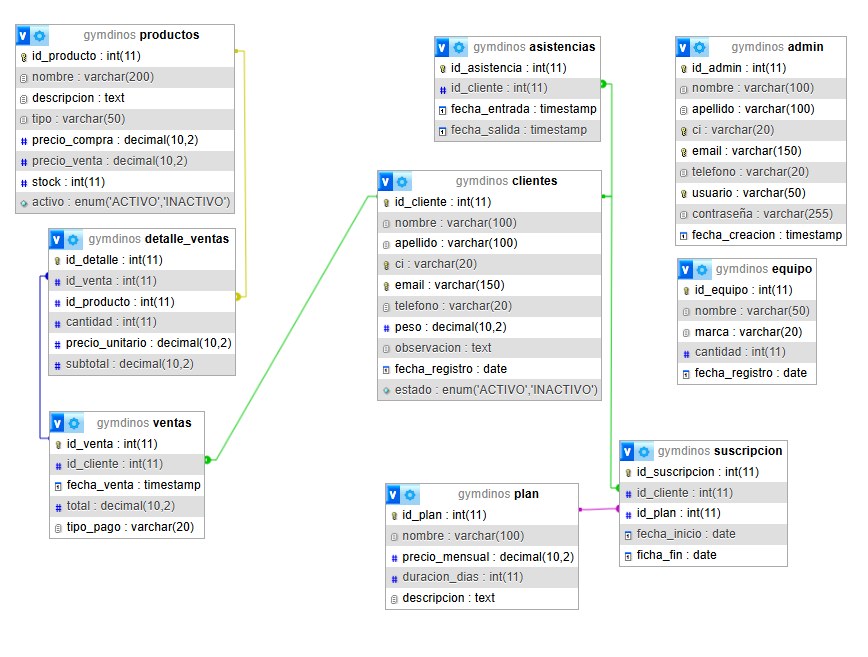
\includegraphics[width=0.8\textwidth]{der.png}
\caption{Diagrama Entidad-Relación de la Base de Datos}
\label{fig:der}
\end{figure}
\newpage

\paragraph{SQL}
\begin{lstlisting}[language=SQL, numbers=left]
CREATE DATABASE dinosgym;
USE dinosgym;
CREATE TABLE admin(
    id_admin INT PRIMARY KEY AUTO_INCREMENT,
    nombre VARCHAR(100) NOT NULL,
    apellido VARCHAR(100) NOT NULL,
    ci VARCHAR(20) UNIQUE NOT NULL,
    email VARCHAR(150) UNIQUE NOT NULL,
    telefono VARCHAR(20),
    usuario VARCHAR(50) UNIQUE NOT NULL,
    contrasena VARCHAR(255) NOT NULL,
    fecha_creacion TIMESTAMP DEFAULT CURRENT_TIMESTAMP
);

CREATE TABLE plan (
    id_plan INT PRIMARY KEY AUTO_INCREMENT,
    nombre VARCHAR(100) NOT NULL,
    precio_mensual DECIMAL(10,2) NOT NULL,
    duracion_dias INT NOT NULL,
    descripcion TEXT
);

CREATE TABLE clientes (
    id_cliente INT PRIMARY KEY AUTO_INCREMENT,
    nombre VARCHAR(100) NOT NULL,
    apellido VARCHAR(100) NOT NULL,
    ci VARCHAR(20) UNIQUE NOT NULL,
    email VARCHAR(150) UNIQUE NOT NULL,
    telefono VARCHAR(20),
    peso DECIMAL(10,2),
    observacion TEXT,
    fecha_registro DATE DEFAULT CURRENT_DATE,
    estado ENUM('ACTIVO', 'INACTIVO') DEFAULT 'ACTIVO'
);

CREATE TABLE productos (
    id_producto INT PRIMARY KEY AUTO_INCREMENT,
    nombre VARCHAR(200) NOT NULL,
    descripcion TEXT,
    tipo VARCHAR(50) NOT NULL,
    precio_compra DECIMAL(10,2) NOT NULL,
    precio_venta DECIMAL(10,2),
    stock INT,
    activo ENUM('ACTIVO', 'INACTIVO') DEFAULT 'ACTIVO'
);

CREATE TABLE equipo(
    id_equipo INT PRIMARY KEY AUTO_INCREMENT,
    nombre VARCHAR(50),
    marca VARCHAR(20),
    cantidad INT NOT NULL,
    fecha_registro DATE DEFAULT CURRENT_DATE
);

CREATE TABLE ventas (
    id_venta INT PRIMARY KEY AUTO_INCREMENT,
    id_cliente INT,
    fecha_venta TIMESTAMP DEFAULT CURRENT_TIMESTAMP,
    total DECIMAL(10,2) NOT NULL,
    tipo_pago VARCHAR(20) NOT NULL,
    FOREIGN KEY (id_cliente) REFERENCES clientes(id_cliente)
);

CREATE TABLE detalle_ventas (
    id_detalle INT PRIMARY KEY AUTO_INCREMENT,
    id_venta INT NOT NULL,
    id_producto INT NOT NULL,
    cantidad INT NOT NULL,
    precio_unitario DECIMAL(10,2) NOT NULL,
    subtotal DECIMAL(10,2) NOT NULL,
    FOREIGN KEY (id_venta) REFERENCES ventas(id_venta),
    FOREIGN KEY (id_producto) REFERENCES productos(id_producto)
);

CREATE TABLE asistencias (
    id_asistencia INT PRIMARY KEY AUTO_INCREMENT,
    id_cliente INT NOT NULL,
    fecha_entrada TIMESTAMP DEFAULT CURRENT_TIMESTAMP,
    fecha_salida TIMESTAMP NULL,
    FOREIGN KEY (id_cliente) REFERENCES clientes(id_cliente)
);

CREATE TABLE suscripcion (
    id_suscripcion INT PRIMARY KEY AUTO_INCREMENT,
    id_cliente INT NOT NULL,
    id_plan INT NOT NULL,
    fecha_inicio DATE NOT NULL,
    ficha_fin DATE NOT NULL,
    FOREIGN KEY (id_cliente) REFERENCES clientes(id_cliente),
    FOREIGN KEY (id_plan) REFERENCES plan(id_plan)
);
\end{lstlisting}
\newpage

\paragraph{Inserción de datos}
\begin{lstlisting}[language=SQL, numbers=left]
INSERT INTO admin (nombre, apellido, ci, email, telefono, usuario, contraseña) VALUES 
('Administrador', 'Sistema', '12345678', 'admin@gimnasio.com', '70123456', 'admin', 'admin');

INSERT INTO plan (nombre, precio_mensual, duracion_dias, descripcion) VALUES
('Plan Básico', 150.00, 30, 'Acceso completo al gimnasio en horarios regulares'),
('Plan Premium', 250.00, 30, 'Acceso completo + clases grupales + nutricionista'),
('Plan VIP', 400.00, 30, 'Acceso 24/7 + entrenador personal + todas las amenidades'),
('Plan Estudiante', 100.00, 30, 'Plan especial para estudiantes con descuento'),
('Plan Anual', 1500.00, 365, 'Plan anual con descuento especial');

INSERT INTO clientes (nombre, apellido, ci, email, telefono, peso, observacion, estado) VALUES
('Juan', 'Pérez', '12345679', 'juan.perez@email.com', '70111111', 75.50, 'Cliente nuevo, objetivos: pérdida de peso', 'ACTIVO'),
('María', 'González', '12345680', 'maria.gonzalez@email.com', '70222222', 62.00, 'Experiencia previa en fitness', 'ACTIVO'),
('Carlos', 'Rodriguez', '12345681', 'carlos.rodriguez@email.com', '70333333', 85.20, 'Enfoque en ganar masa muscular', 'ACTIVO'),
('Ana', 'López', '12345682', 'ana.lopez@email.com', '70444444', 58.75, 'Rehabilitación de lesión de rodilla', 'ACTIVO'),
('Pedro', 'Mamani', '12345683', 'pedro.mamani@email.com', '70555555', 90.00, 'Cliente avanzado', 'ACTIVO'),
('Lucia', 'Fernández', '12345684', 'lucia.fernandez@email.com', '70666666', 55.30, NULL, 'INACTIVO');

INSERT INTO productos (nombre, descripcion, tipo, precio_compra, precio_venta, stock, activo) VALUES
('Proteína Whey 2kg', 'Proteína en polvo sabor vainilla', 'Suplemento', 180.00, 250.00, 25, 'ACTIVO'),
('Creatina 300g', 'Creatina monohidratada pura', 'Suplemento', 80.00, 120.00, 15, 'ACTIVO'),
('Shaker 500ml', 'Vaso mezclador con compartimentos', 'Accesorio', 15.00, 35.00, 50, 'ACTIVO'),
('Toalla Deportiva', 'Toalla de microfibra absorbente', 'Accesorio', 25.00, 45.00, 30, 'ACTIVO'),
('Guantes de Entrenamiento', 'Guantes acolchados para levantamiento', 'Accesorio', 35.00, 65.00, 20, 'ACTIVO'),
('Pre-Workout 250g', 'Suplemento pre-entreno con cafeína', 'Suplemento', 90.00, 150.00, 12, 'ACTIVO'),
('Aminoácidos BCAA', 'Aminoácidos ramificados en cápsulas', 'Suplemento', 70.00, 110.00, 8, 'INACTIVO');

INSERT INTO equipo (nombre, marca, cantidad) VALUES
('Caminadora', 'TechnoGym', 5),
('Bicicleta Estática', 'Life Fitness', 8),
('Elíptica', 'Matrix', 4),
('Banco Press Plano', 'Hammer Strength', 6),
('Rack de Sentadillas', 'Rogue', 3),
('Mancuernas', 'York', 50),
('Barras Olímpicas', 'Eleiko', 10),
('Máquina Multiestación', 'Cybex', 2);

INSERT INTO ventas (id_cliente, total, tipo_pago) VALUES
(1, 285.00, 'EFECTIVO'),
(2, 120.00, 'TARJETA'),
(3, 65.00, 'EFECTIVO'),
(1, 45.00, 'QR'),
(4, 150.00, 'TARJETA');

INSERT INTO detalle_ventas (id_venta, id_producto, cantidad, precio_unitario, subtotal) VALUES
-- Venta 1 (Juan): Proteína + Shaker
(1, 1, 1, 250.00, 250.00),
(1, 3, 1, 35.00, 35.00),
-- Venta 2 (María): Creatina
(2, 2, 1, 120.00, 120.00),
-- Venta 3 (Carlos): Guantes
(3, 5, 1, 65.00, 65.00),
-- Venta 4 (Juan): Toalla
(4, 4, 1, 45.00, 45.00),
-- Venta 5 (Ana): Pre-workout
(5, 6, 1, 150.00, 150.00);

INSERT INTO suscripcion (id_cliente, id_plan, fecha_inicio, ficha_fin) VALUES
(1, 1, '2024-09-01', '2024-10-01'),  -- Juan - Plan Básico
(2, 2, '2024-09-15', '2024-10-15'),  -- María - Plan Premium  
(3, 3, '2024-09-10', '2024-10-10'),  -- Carlos - Plan VIP
(4, 4, '2024-09-20', '2024-10-20'),  -- Ana - Plan Estudiante
(5, 1, '2024-09-05', '2024-10-05'),  -- Pedro - Plan Básico
(6, 2, '2024-08-01', '2024-09-01');  -- Lucia - Plan Premium (vencido)

INSERT INTO asistencias (id_cliente, fecha_entrada, fecha_salida) VALUES
(1, '2024-09-25 08:30:00', '2024-09-25 10:00:00'),
(2, '2024-09-25 09:15:00', '2024-09-25 10:45:00'),
(3, '2024-09-25 18:00:00', '2024-09-25 19:30:00'),
(1, '2024-09-24 07:45:00', '2024-09-24 09:15:00'),
(4, '2024-09-24 16:30:00', '2024-09-24 18:00:00'),
(5, '2024-09-26 06:00:00', NULL),
(2, '2024-09-26 19:00:00', NULL),
(3, '2024-09-23 17:00:00', '2024-09-23 18:30:00');
\end{lstlisting}
\newpage

\paragraph{Sistema de gestión} 
El sistema está montado con una interfaz gráfica desarrollada en HTML, CSS, y la base de datos está implementada en MySQL.\\
\textbf{Admin}
\begin{figure}[ht]
\centering
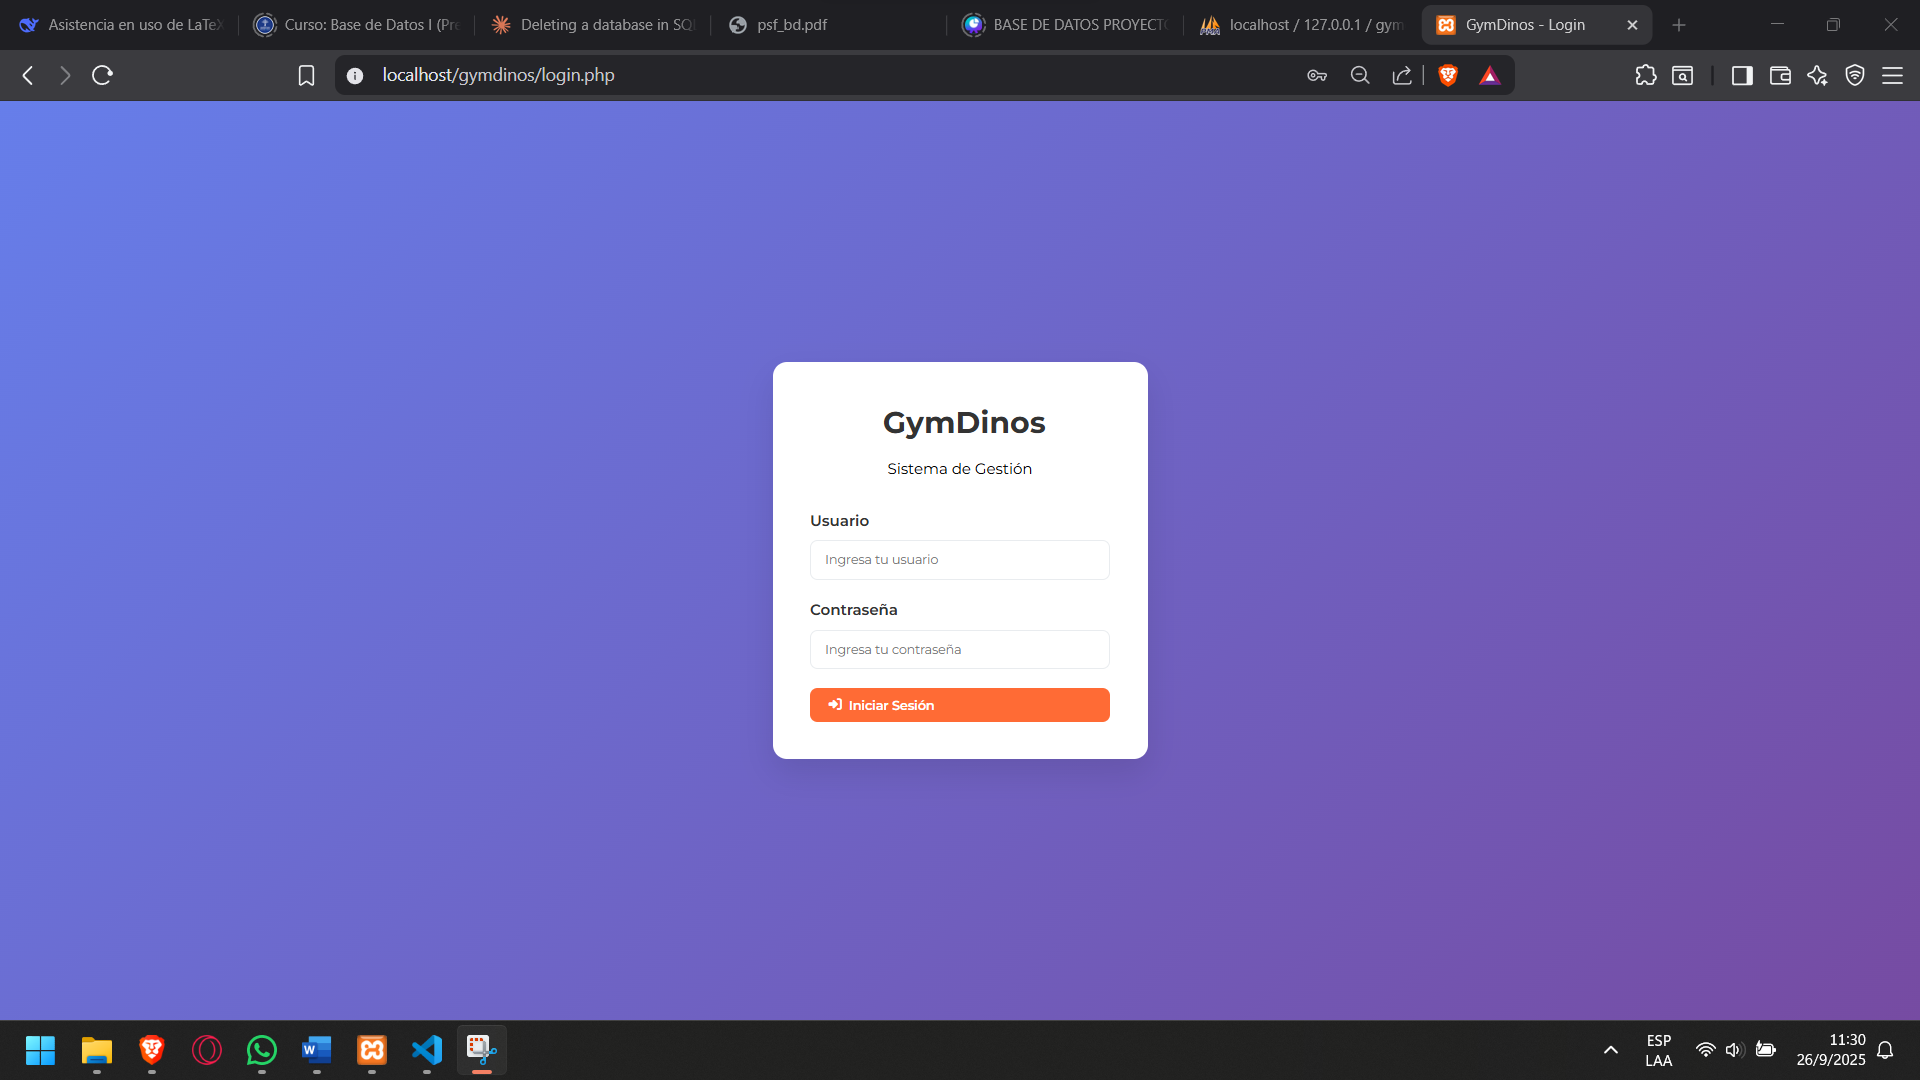
\includegraphics[width=0.8\textwidth]{admin.png}
\caption{Interfaz de Administración del Sistema}
\label{fig:admin}
\end{figure}

\textbf{Dashboard}
\begin{figure}[ht]
\centering
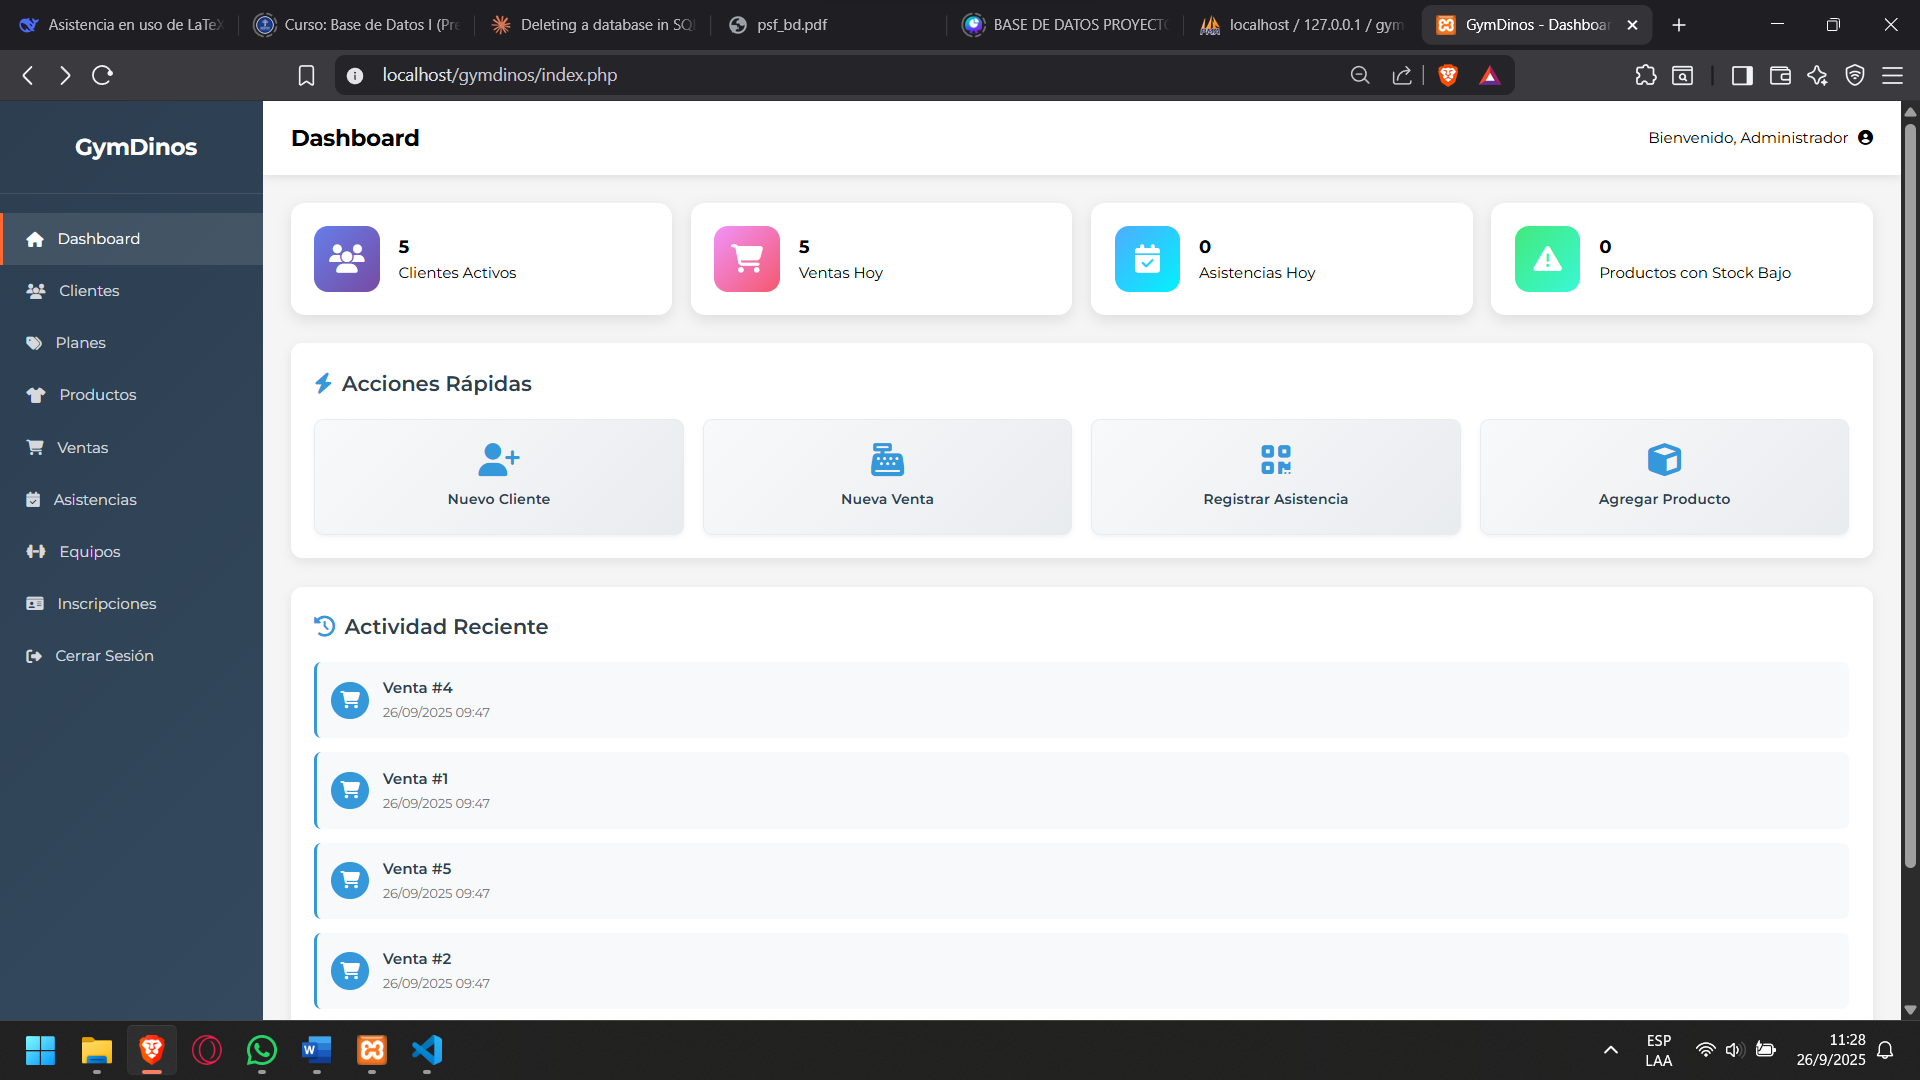
\includegraphics[width=0.8\textwidth]{dashboard.png}
\caption{Dashboard Principal del Sistema}
\label{fig:dashboard}
\end{figure}
\newpage

\textbf{Clientes}
\begin{figure}[ht]
\centering
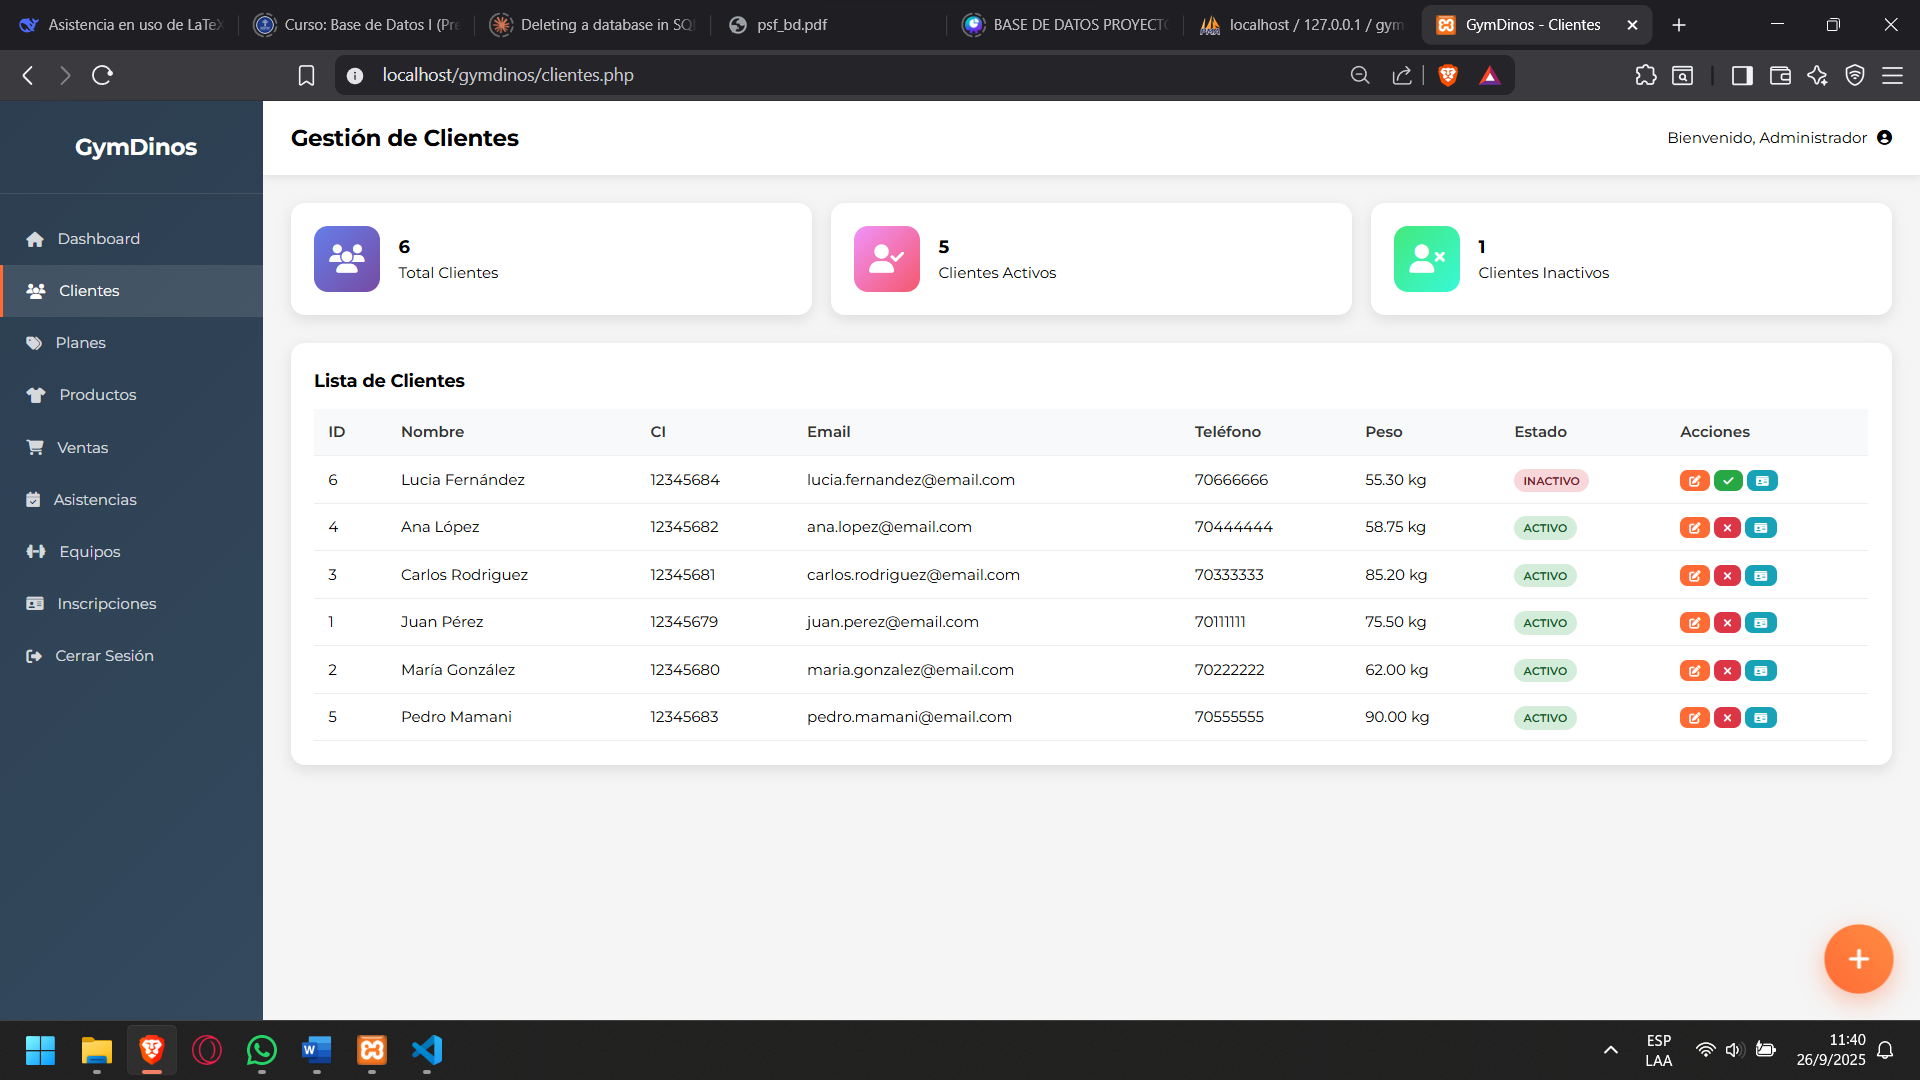
\includegraphics[width=0.8\textwidth]{clientes.png}
\caption{Gestión de Clientes}
\label{fig:clientes}
\end{figure}

\textbf{Planes}
\begin{figure}[ht]
\centering
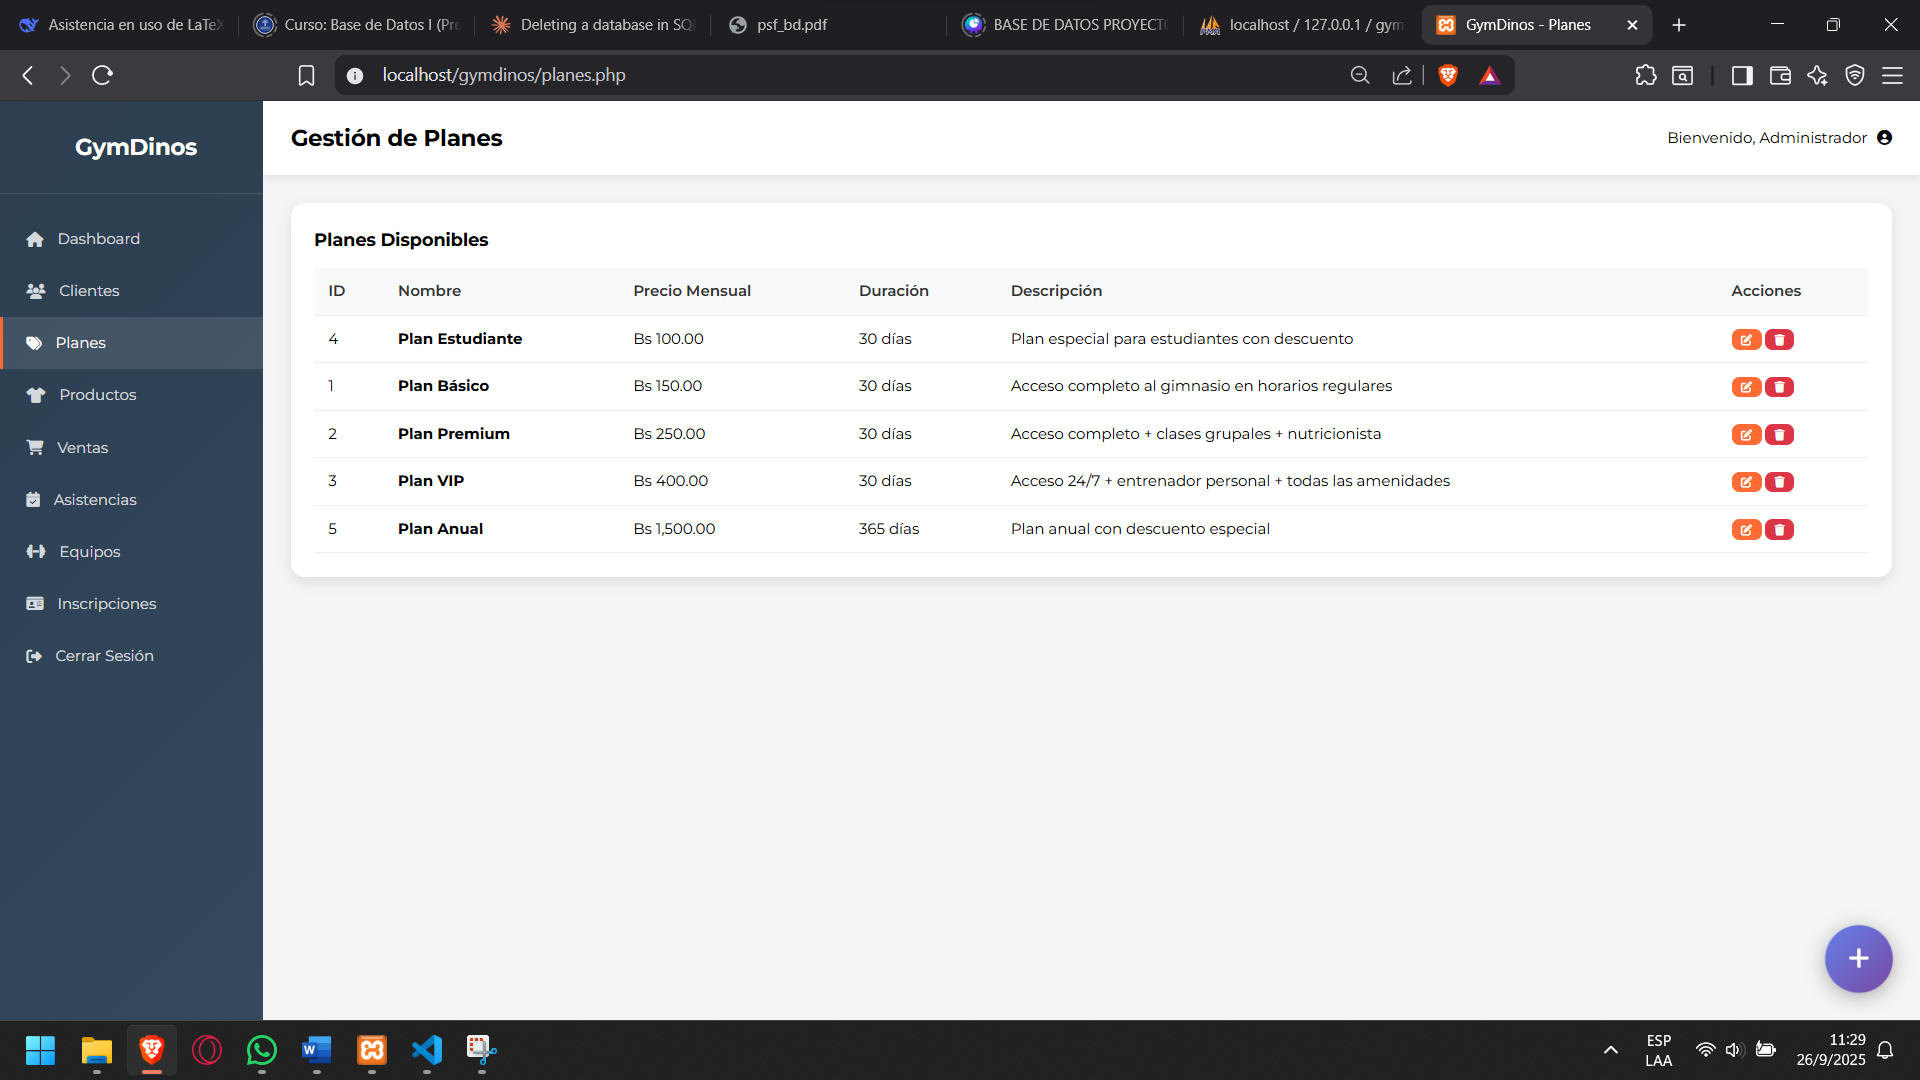
\includegraphics[width=0.8\textwidth]{planes.png}
\caption{Gestión de Planes de Membresía}
\label{fig:planes}
\end{figure}
\newpage

\textbf{Productos}
\begin{figure}[ht]
\centering
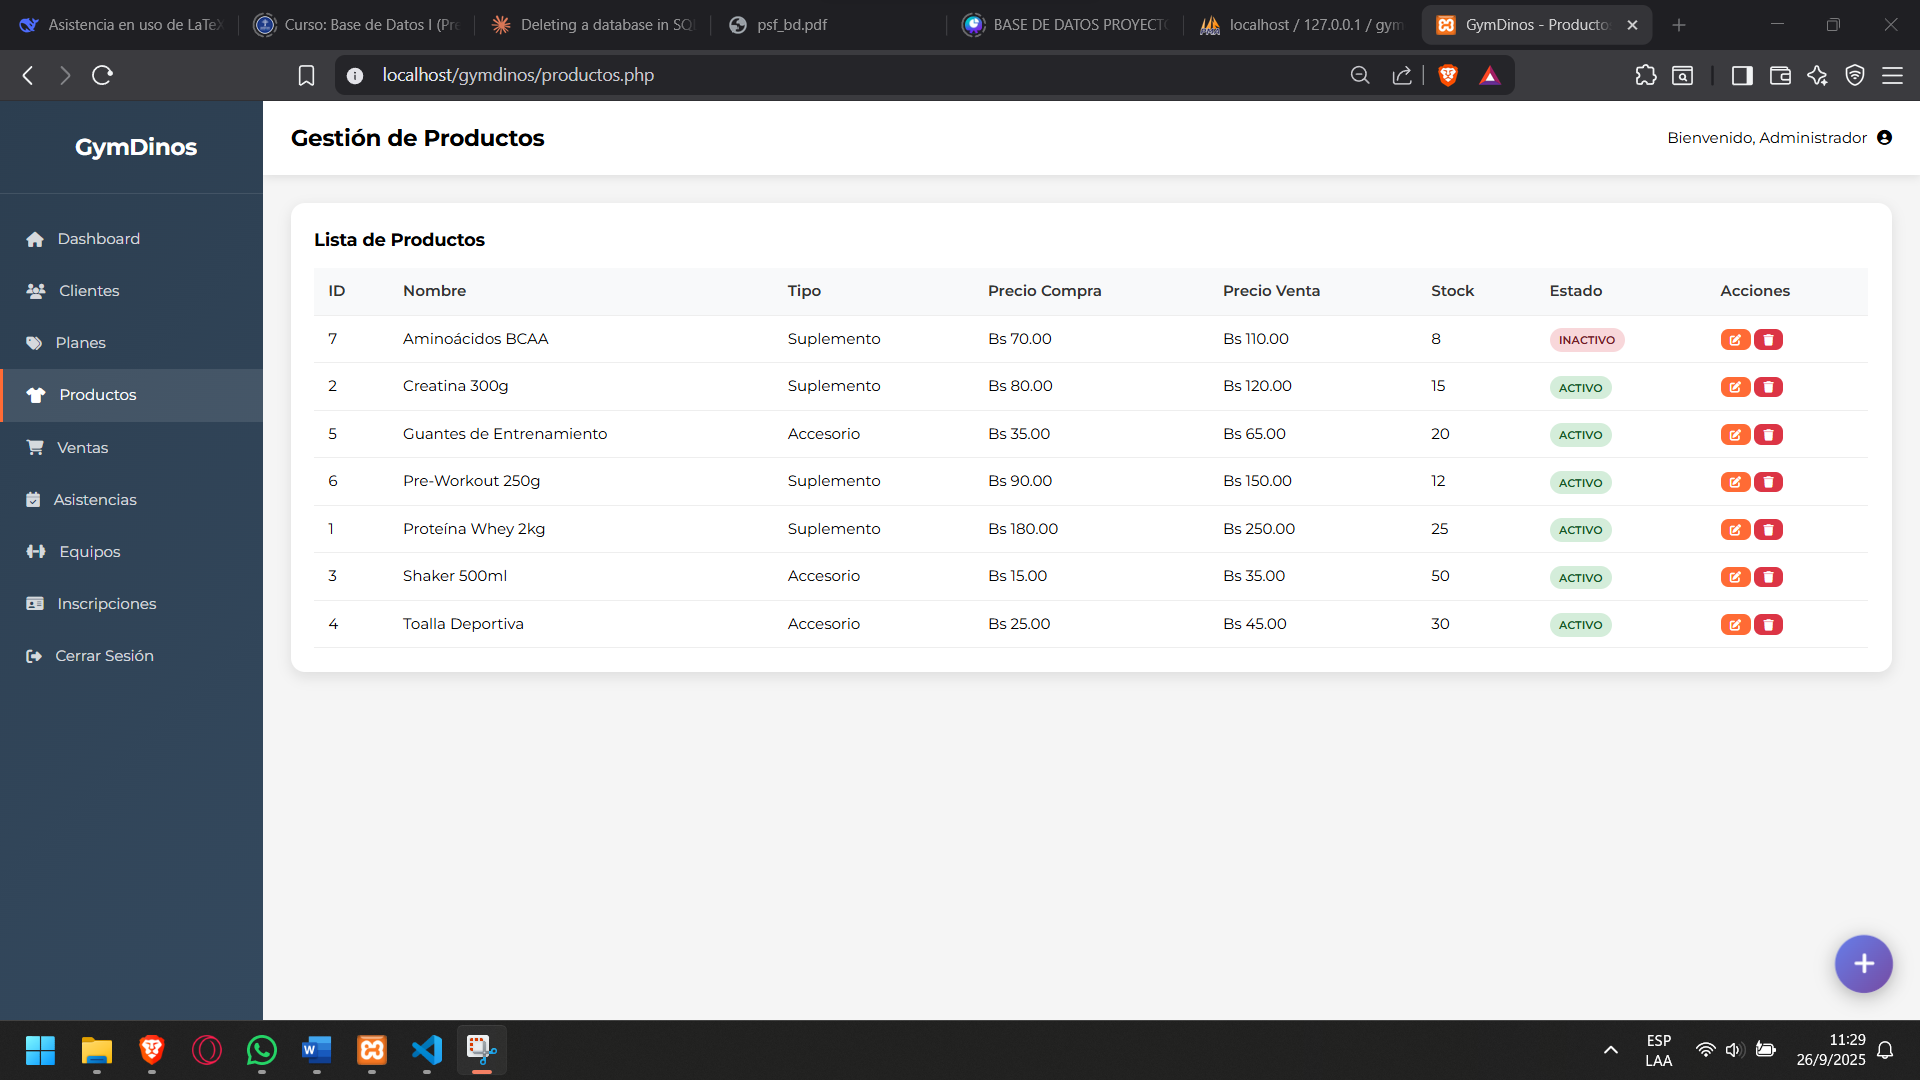
\includegraphics[width=0.8\textwidth]{productos.png}
\caption{Gestión de Productos y Suplementos}
\label{fig:productos}
\end{figure}

\textbf{Ventas}
\begin{figure}[ht]
\centering
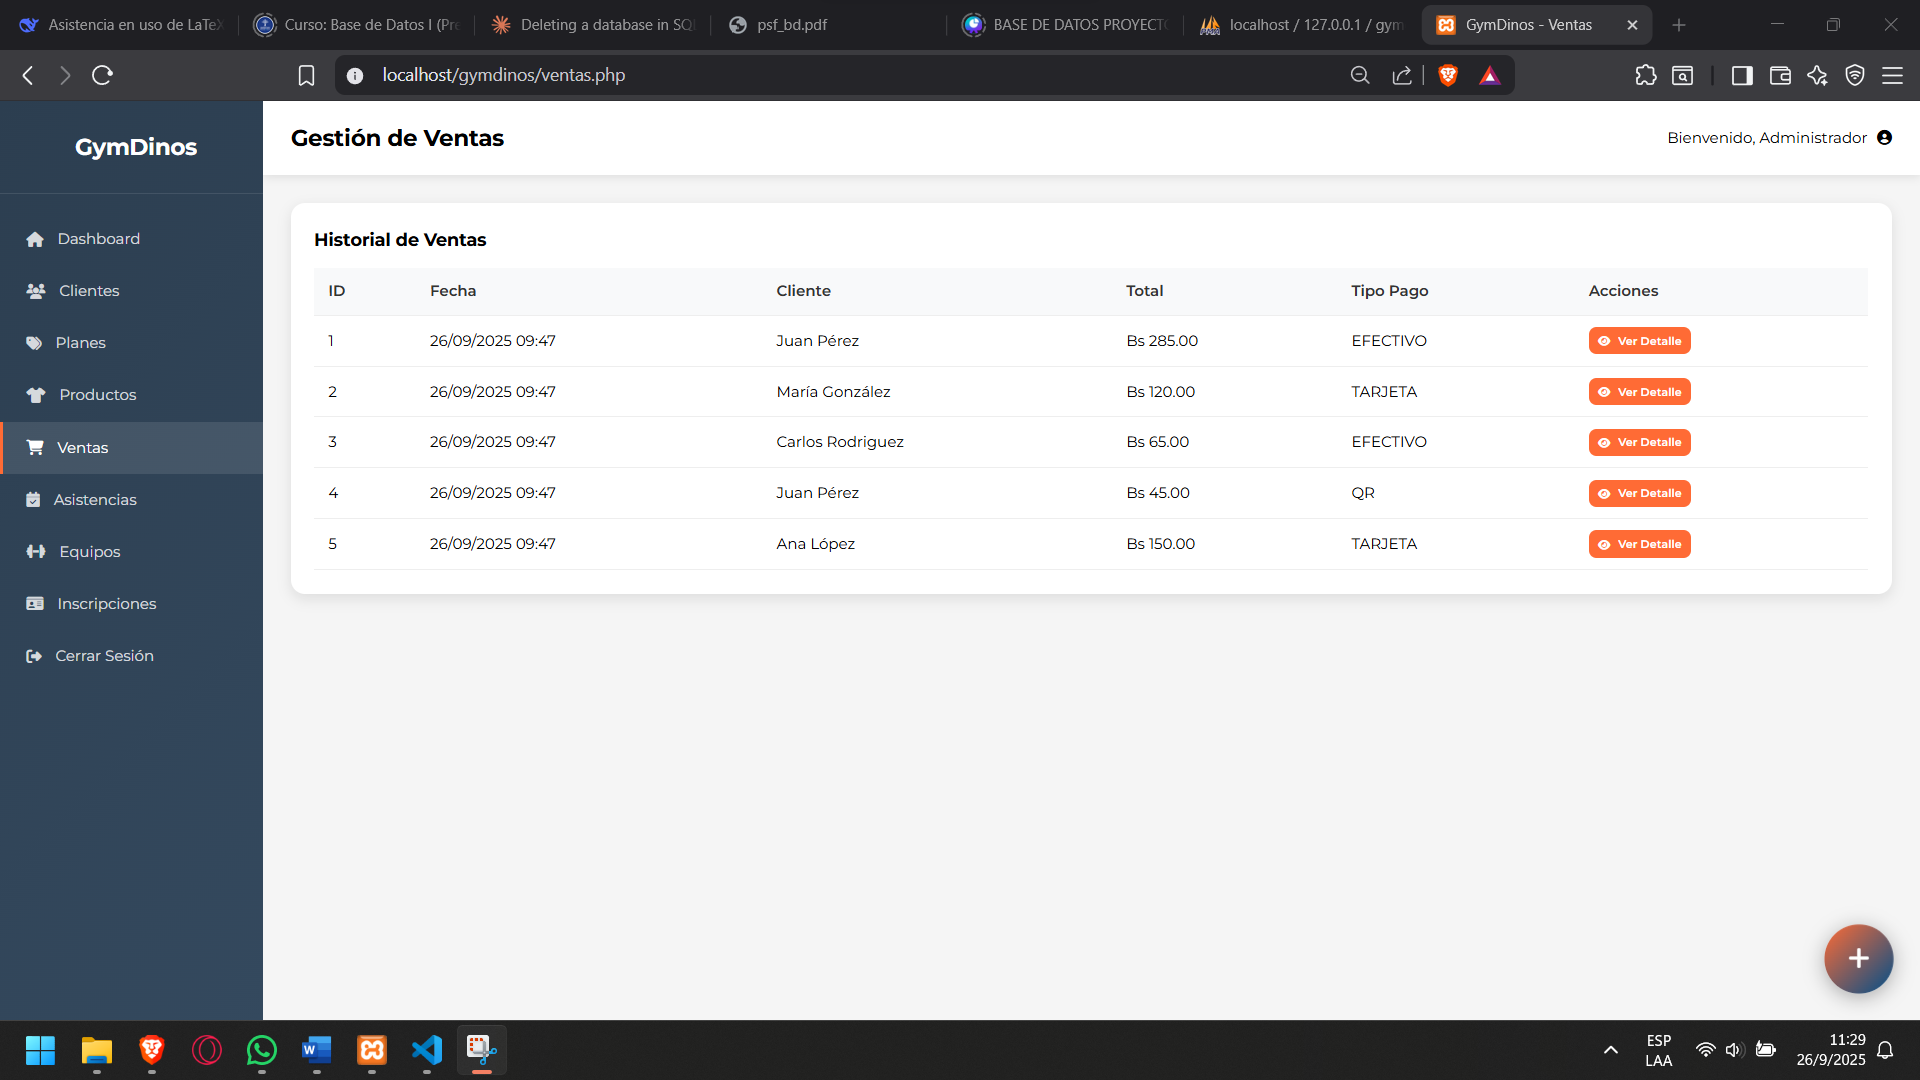
\includegraphics[width=0.8\textwidth]{ventas.png}
\caption{Registro de Ventas}
\label{fig:ventas}
\end{figure}
\newpage

\textbf{Asistencias}
\begin{figure}[ht]
\centering
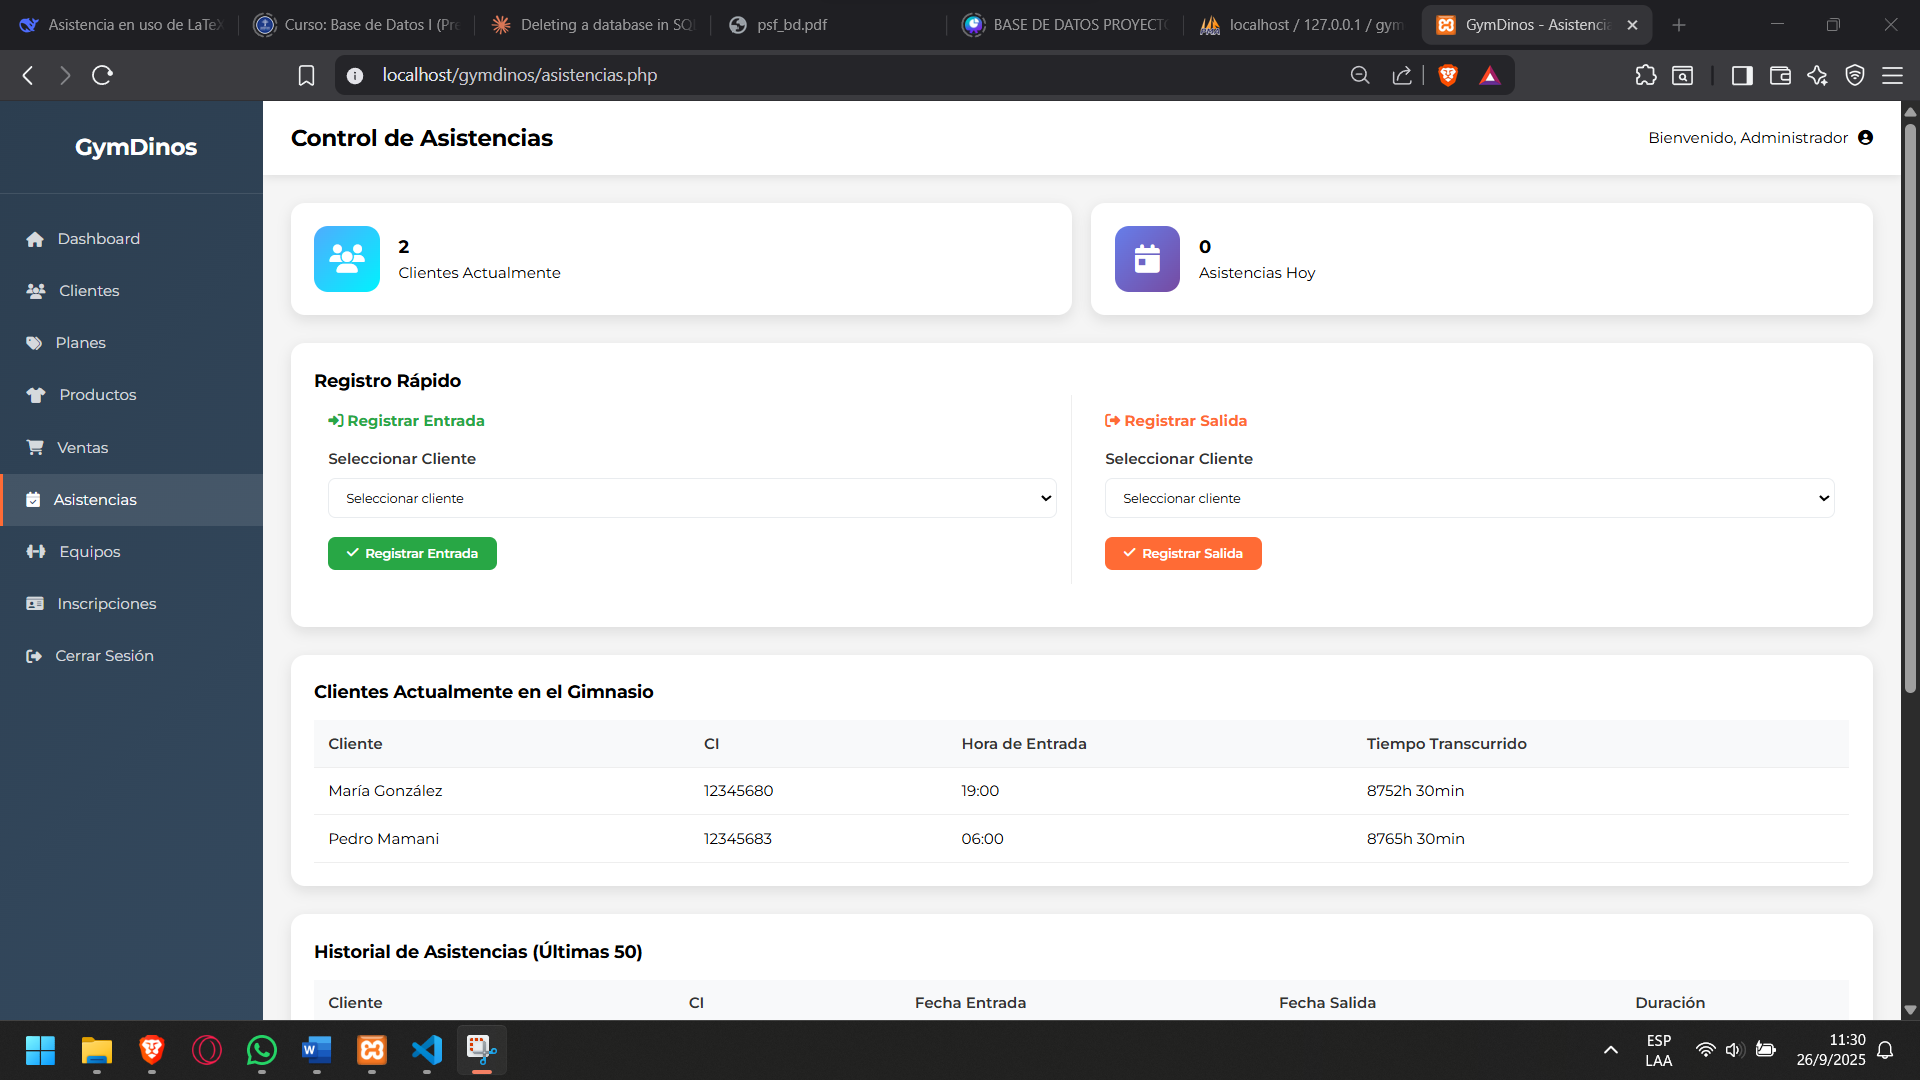
\includegraphics[width=0.8\textwidth]{asistencias.png}
\caption{Control de Asistencias}
\label{fig:asistencias}
\end{figure}

\textbf{Equipos}
\begin{figure}[ht]
\centering
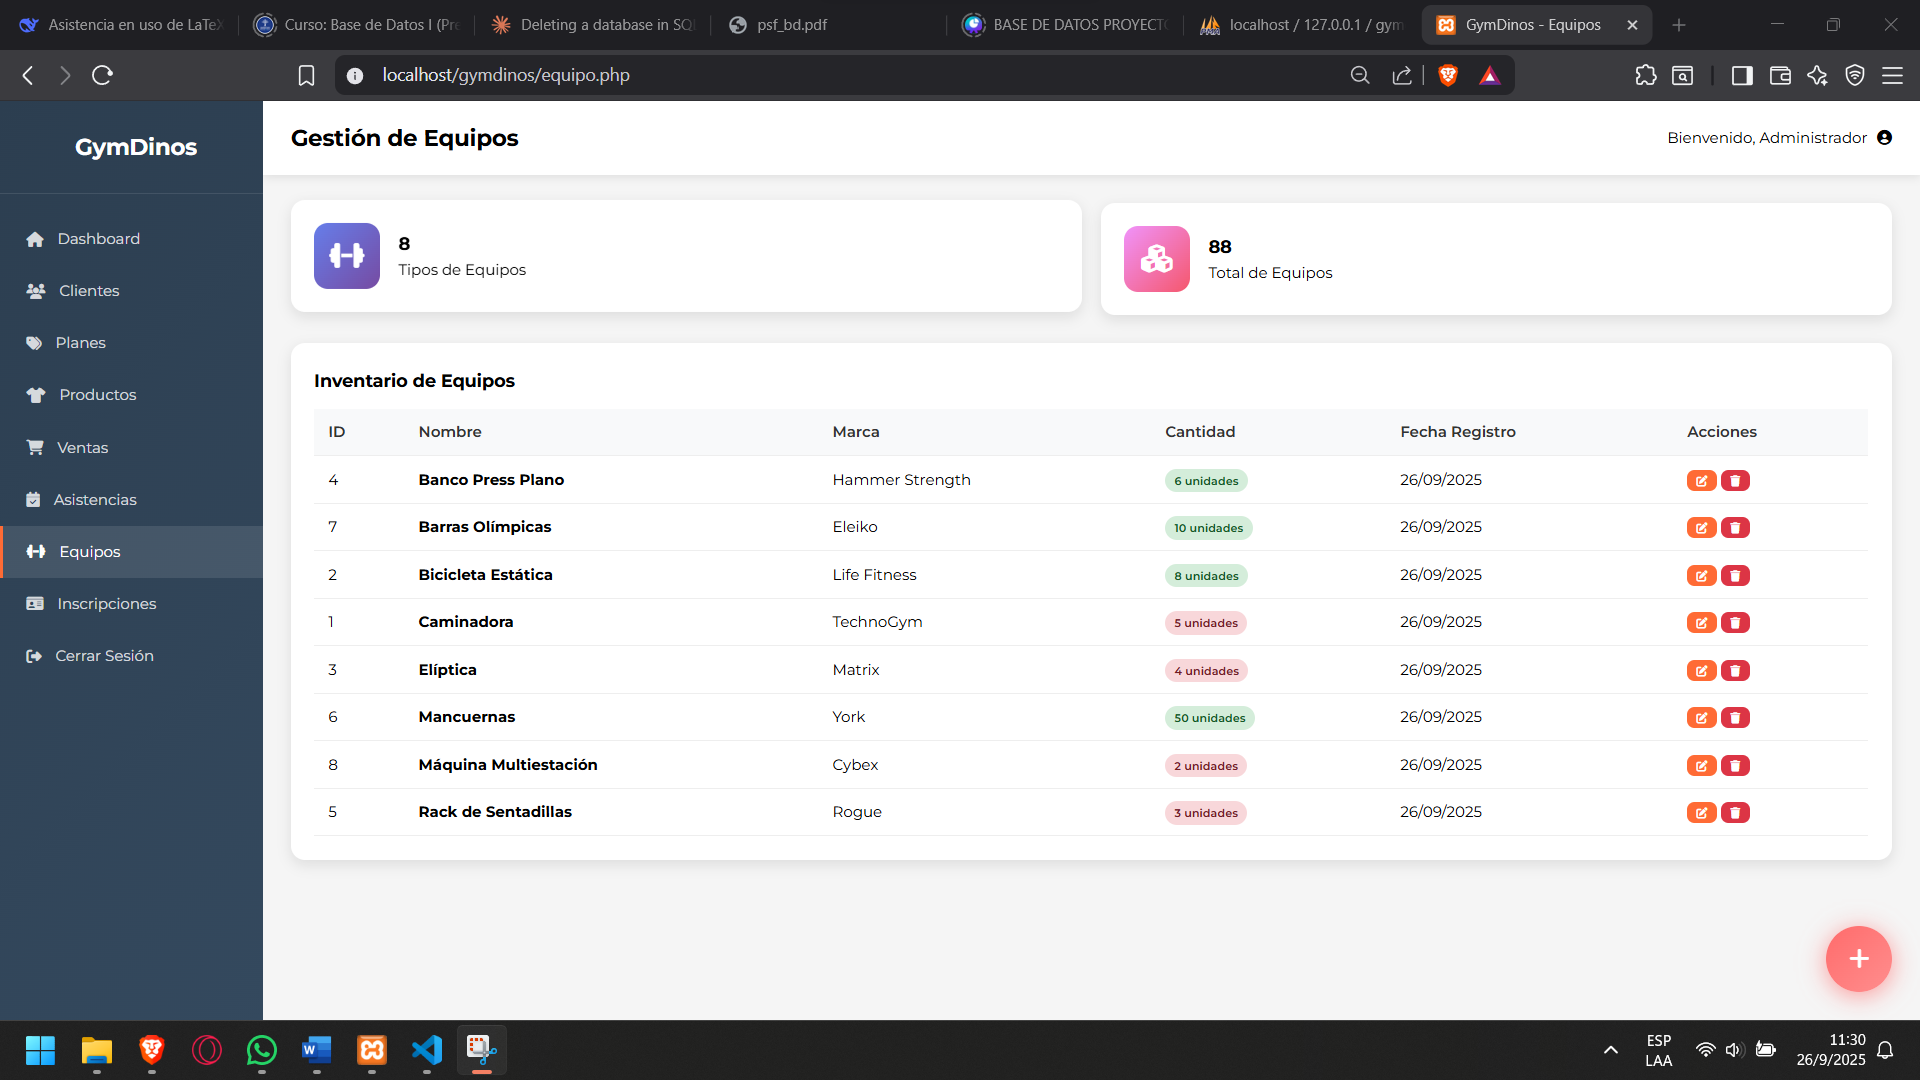
\includegraphics[width=0.8\textwidth]{equipos.png}
\caption{Gestión de Equipos del Gimnasio}
\label{fig:equipos}
\end{figure}
\newpage

\textbf{Inscripciones}
\begin{figure}[ht]
\centering
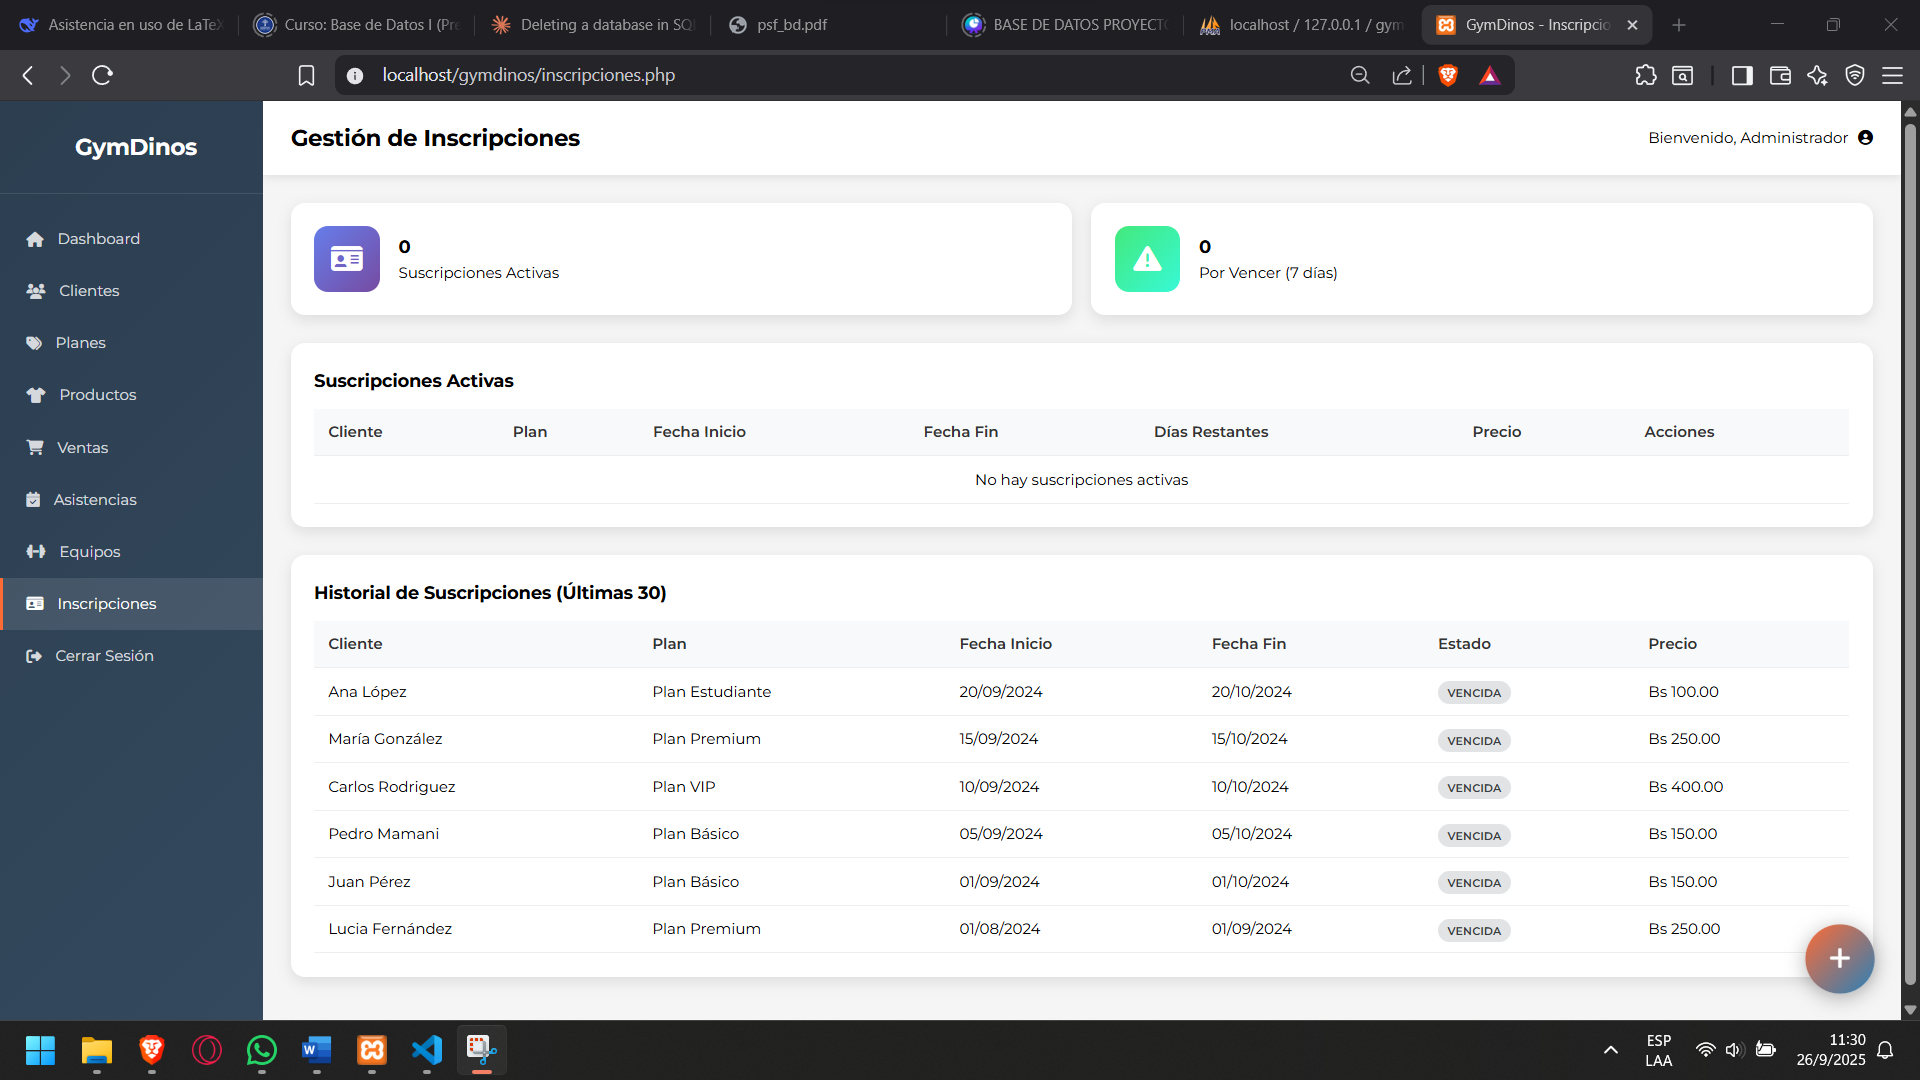
\includegraphics[width=0.8\textwidth]{inscripciones.png}
\caption{Proceso de Inscripción de Clientes}
\label{fig:inscripciones}
\end{figure}
\newpage

\section*{CAPÍTULO IV}
\addcontentsline{toc}{section}{CAPÍTULO IV}
\setcounter{section}{4}
\subsection{CONCLUSIONES Y RECOMENDACIONES}
\subsubsection{Conclusiones}
La implementación del sistema de base de datos para DINOS GYM ha demostrado ser una solución integral que responde efectivamente a las necesidades identificadas en el análisis inicial.\\ 
A partir de los objetivos específicos planteados, se pueden establecer las siguientes conclusiones:
\paragraph{En relación al análisis de requerimientos funcionales y de información:}
Se identificaron exitosamente los requerimientos críticos del gimnasio, incluyendo la necesidad de gestionar información detallada de socios, control de asistencia automatizado, seguimiento de pagos y membresías, y generación de reportes automáticos. El análisis reveló que la base de datos anterior presentaba limitaciones significativas en términos de escalabilidad, seguridad y capacidad de reporting, lo cual justificó plenamente la necesidad de implementar una solución más robusta.
\paragraph{Respecto al diseño del modelo de datos:}
El modelo relacional desarrollado integra de manera coherente las entidades principales del negocio: clientes, planes, productos, ventas, asistencias, equipos y suscripciones. La aplicación de principios de normalización hasta la tercera forma normal garantiza la eliminación de redundancias y mantiene la integridad referencial. Las relaciones establecidas entre las tablas permiten consultas eficientes y reportes completos, facilitando la toma de decisiones basada en datos confiables.
\paragraph{En cuanto a la implementación en MySQL:}
La estructura de base de datos creada en MySQL proporciona un entorno estable y seguro para el manejo de la información. La implementación incluye restricciones de integridad, claves foráneas apropiadas y tipos de datos optimizados para cada campo. El sistema permite el almacenamiento eficiente de grandes volúmenes de información y facilita las operaciones de consulta, inserción, actualización y eliminación de datos.
\paragraph{Sobre la optimización del procesamiento de consultas:}
El diseño implementado permite un procesamiento más ágil de las consultas mediante la correcta indexación de campos clave, la estructura normalizada de las tablas y la definición adecuada de relaciones. Las consultas para generar reportes de asistencia, estados de membresías y análisis de ventas se ejecutan de manera eficiente, reduciendo significativamente los tiempos de respuesta comparados con el sistema anterior.
\paragraph{Impacto general del proyecto:}
La implementación del nuevo sistema de base de datos representa una mejora sustancial en la capacidad operativa de DINOS GYM. El sistema permite la automatización de procesos previamente manuales, reduce la posibilidad de errores humanos, facilita el acceso rápido a información crítica y proporciona herramientas de análisis que apoyan la gestión estratégica del negocio. Además, la escalabilidad del sistema asegura que pueda adaptarse al crecimiento futuro del gimnasio.

\subsubsection{Recomendaciones}
Basándose en la experiencia obtenida durante el desarrollo e implementación del sistema, se formulan las siguientes recomendaciones para maximizar los beneficios de la solución implementada:\\
\paragraph{Respaldos y seguridad:}
Es crucial establecer un protocolo robusto de respaldos automáticos diarios de la base de datos, con copias de seguridad almacenadas tanto localmente como en servicios de almacenamiento en la nube. Se recomienda implementar medidas adicionales de seguridad como autenticación de dos factores para administradores y encriptación de datos sensibles.\\
\paragraph{Expansión funcional:}
Para futuras mejoras, se recomienda considerar la integración de funcionalidades adicionales como un módulo de comunicación con clientes (notificaciones automáticas de vencimiento de membresías), sistema de reserva de clases grupales, integración con dispositivos de control de acceso biométrico, y desarrollo de una aplicación móvil para clientes.\\
\paragraph{Análisis de datos:}
Aprovechar la capacidad de reporting del sistema para generar análisis regulares de tendencias de asistencia, patrones de consumo, efectividad de planes de membresía y satisfacción del cliente. Esta información debe utilizarse para tomar decisiones estratégicas sobre precios, horarios de operación, adquisición de equipos y desarrollo de nuevos servicios.\\ \\
La implementación exitosa de estas recomendaciones asegurará que el sistema de base de datos para DINOS GYM continúe proporcionando valor agregado al negocio y se mantenga como una herramienta efectiva para la gestión integral del gimnasio.
\newpage

\section*{BIBLIOGRAFÍA}
\addcontentsline{toc}{section}{BIBLIOGRAFÍA}
\setcounter{section}{5}

\begin{thebibliography}{99}

\bibitem{ordonez2019} 
Ordoñez Molina, J. (2019). \textit{Diseño e implementación de un sistema de información para ingreso de Usuario de Gym Elite}. Universidad Técnica de Ambato.

\bibitem{andrich2021}
Andrich, A., Briceño, M., \& Dirie, H. (2021). \textit{Sistema de Gestión de Gimnasios}. Universidad Centroccidental Lisandro Alvarado.

\bibitem{codest2021}
Codest. (2021). \textit{Diseño de bases de datos relacionales}. Recuperado de https://www.codest.com/blog/diseno-bases-datos-relacionales

\bibitem{rodriguez2023}
Rodriguez, M. (2023). \textit{GymTEC: Sistema de gestión integral para gimnasios}. Revista de Tecnología e Innovación, 15(2), 45-62.

\bibitem{ortega2025}
Ortega, P. (2025). \textit{Métodos de investigación cuantitativa}. Editorial Académica.

\bibitem{muguira2023}
Muguira, J. (2023). \textit{Investigación descriptiva: Fundamentos y aplicaciones}. Revista de Metodología de la Investigación, 8(1), 23-45.

\bibitem{etece2024}
Etecé. (2024). \textit{Método analítico}. En DeConceptos.com. Recuperado de https://deconceptos.com/ciencias-sociales/metodo-analitico

\bibitem{narvaez2022}
Narvaez, R. (2022). \textit{El método deductivo en la investigación científica}. Revista de Epistemología, 12(3), 78-95.

\bibitem{ioe2024}
IOE. (2024). \textit{Método inductivo: De lo particular a lo general}. Instituto de Orientación Educativa.

\bibitem{muguira2023obs}
Muguira, A. (2023). \textit{Técnicas de observación en investigación cualitativa}. Revista de Métodos de Investigación, 7(2), 112-128.

\bibitem{mendez2010}
Mendez, C. (2010). \textit{Metodología de la investigación}. McGraw-Hill.

\bibitem{definicion2024}
Definición.de. (2024). \textit{Guía de observación}. Recuperado de https://definicion.de/guia-de-observacion/

\bibitem{farias2025}
Farías, M. (2025). \textit{Elaboración de fichas bibliográficas}. Manual de Investigación Documental.

\bibitem{laudon2022}
Laudon, K. C., \& Laudon, J. P. (2022). \textit{Sistemas de información gerencial} (16ª ed.). Pearson Education.

\bibitem{openwebinars2022}
OpenWebinars. (2022). \textit{Cómo realizar la normalización de bases de datos y por qué}. Recuperado de https://openwebinars.net/blog/como-realizar-la-normalizacion-de-bases-de-datos-y-por-que/

\bibitem{microsoft2024}
Microsoft. (2024). \textit{Fundamentos de la normalización de bases de datos}. Recuperado de https://learn.microsoft.com/es-es/office/troubleshoot/access/database-normalization-description

\bibitem{freecodecamp2023}
FreeCodeCamp. (2023). \textit{Normalización de base de datos: formas normales 1NF 2NF 3NF ejemplos de tablas}. Recuperado de https://www.freecodecamp.org/espanol/news/normalizacion-de-base-de-datos-formas-normales-1nf-2nf-3nf-ejemplos-de-tablas/

\bibitem{trainingym2024}
Trainingym. (2024). \textit{Tendencias tecnológicas en la industria del fitness 2024}. Recuperado de https://blog.trainingym.com/es/blog/tendencias-tecnologicas-en-la-industria-del-fitness-2025

\bibitem{softwarepara2025}
SoftwarePara. (2025). \textit{Software para gimnasios: 8 grandes programas de gestión}. Recuperado de https://softwarepara.net/gimnasios/

\bibitem{clupik2022}
Clupik. (2022). \textit{Cómo elegir el mejor CRM para tu organización deportiva}. Recuperado de https://clupik.com/blog/crm-club-deportivo/

\bibitem{resamania2024}
Resamania. (2024). \textit{Usar la base de datos de socios de su gimnasio para marcar objetivos relevantes}. Recuperado de https://resamania.es/blog/usar-base-de-datos-socios-gimnasio-objetivos-relevantes/

\bibitem{avigilon2023}
Avigilon. (2023). \textit{Guía de sistemas de control de acceso 24/7 para gimnasios}. Recuperado de https://www.avigilon.com/es/blog/gym-access-control

\bibitem{apachefriends2024}
Apache Friends. (2024). \textit{XAMPP Apache + MariaDB + PHP + Perl}. Recuperado de https://www.apachefriends.org/index.html

\bibitem{mozillahtml2024}
Mozilla Developer Network. (2024). \textit{HTML: Lenguaje de etiquetas de hipertexto}. Recuperado de https://developer.mozilla.org/es/docs/Web/HTML

\bibitem{mozillacss2024}
Mozilla Developer Network. (2024). \textit{CSS: Hojas de Estilo en Cascada}. Recuperado de https://developer.mozilla.org/es/docs/Web/CSS

\bibitem{coronel2017}
Coronel, C., \& Morris, S. (2017). \textit{Database Systems: Design, Implementation, and Management} (12ª ed.). Cengage Learning.

\bibitem{silberschatz2018}
Silberschatz, A., Galvin, P. B., \& Gagne, G. (2018). \textit{Operating System Concepts} (10ª ed.). John Wiley \& Sons.

\bibitem{lamport2023}
Lamport, L. (2023). \textit{LaTeX: A Document Preparation System} (2ª ed.). Addison-Wesley Professional.

\bibitem{oetiker2024}
Oetiker, T., Partl, H., Hyna, I., \& Schlegl, E. (2024). \textit{The Not So Short Introduction to LaTeX2e}. Recuperado de https://tobi.oetiker.ch/lshort/lshort.pdf

\end{thebibliography}

%\section*{ANEXOS}
%\addcontentsline{toc}{section}{ANEXOS}
%\setcounter{section}{6}
\end{document}